%\documentstyle[aas2pp4,epsf]{article}
%%%\documentstyle[aaspp4,epsf]{article}
%\documentstyle[12pt,aasms]{article}    % this is for a preprint
%(single-spaced)
%\documentstyle[aaspp4,epsf]{article} % this is for small print
%\documentstyle[12pt, aaspp4]{article}

%\documentstyle[11pt,aaspp]{article}
%\documentclass[12pt, preprint]{aastex} 

%\documentclass[manuscript]{aastex}
\documentclass[apj]{emulateapj}

%\documentclass[12pt, preprint,numberedappendix]{emulateapj}
%\documentstyle[12pt,aasms]{article}    % this is for submittal
                                       % (double-spaced)

%\documentstyle[12pt,aasms]{article}   \usepackage{emulateapj5} 

\usepackage{graphicx} 
\usepackage{graphics}                       
\usepackage{amsmath}
\usepackage{hyperref}
\usepackage{amsfonts}
\usepackage{amsmath}
\usepackage{amssymb}
\usepackage{amsthm}
\usepackage{subeqnarray}
%\bibliographystyle{apj}

\newcommand{\delad}{\nabla_{\rm ad}}
\newcommand{\delrad}{\nabla_{\rm rad}}
\newcommand{\emgr}[1]{\emph{ \color{gray} #1}}

\newcommand{\ie}{i.e.\ }
\newcommand{\eg}{e.g.\ }
\newcommand{\p}{\partial}
\newcommand{\xv}{\vc{x}}
\newcommand{\kv}{\vc{k}}
\newcommand{\brak}[1]{\langle #1\rangle}


\newcommand{\gcc}{\;\mathrm{g\; cm^{-3}}}
\newcommand{\gsc}{\;\mathrm{g\; cm^{-2}}}
\newcommand{\cm}{\; {\rm cm}}
\newcommand{\mm}{\; {\rm mm}}
%\newcommand{\ps}{\; {\rm s^{-1}}}
\newcommand{\km}{\; {\rm km}}
%\newcommand{\au}{\; \varpi_{\rm AU}}

\newcommand{\AU}{\; {\rm AU}}
\newcommand{\yr}{\; {\rm yr}}
\def\K{\; {\rm K}}

\newcommand{\vcs}[1]{\mbox{\boldmath{$\scriptstyle{#1}$}}}
\newcommand{\vc}[1]{\mbox{\boldmath{$#1$}}}
\newcommand{\nab}{\vc{\nabla}}
\DeclareMathSymbol{\varOmega}{\mathord}{letters}{"0A}
\DeclareMathSymbol{\varSigma}{\mathord}{letters}{"06}
\DeclareMathSymbol{\varPsi}{\mathord}{letters}{"09}

\newcommand{\Eq}[1]{Equation\,(\ref{#1})}
\newcommand{\Eqs}[2]{Equations (\ref{#1}) and~(\ref{#2})}
\newcommand{\Eqss}[2]{Equations (\ref{#1})--(\ref{#2})}
\newcommand{\Eqsss}[3]{Equations (\ref{#1}), (\ref{#2}) and~(\ref{#3})}
\newcommand{\App}[1]{Appendix~\ref{#1}}
\newcommand{\Sec}[1]{Sect.~\ref{#1}}
\newcommand{\Chap}[1]{Chapter~\ref{#1}}
\newcommand{\Fig}[1]{Fig.~\ref{#1}}
\newcommand{\Figs}[2]{Figs.~\ref{#1} and \ref{#2}}
\newcommand{\Figss}[2]{Figs.~\ref{#1}--\ref{#2}} 
\newcommand{\Tab}[1]{Table \ref{#1}}

\newenvironment{packed_item}{
\begin{itemize}
  \setlength{\itemsep}{1pt}
  \setlength{\parskip}{0pt}
  \setlength{\parsep}{0pt}
}{\end{itemize}}

%\newcommand{\delad}{\nabla_{\rm ad}}
%\newcommand{\delrad}{\nabla_{\rm rad}}
\newcommand{\Rg}{\mathcal{R}}
\newcommand{\RB}{R_{\rm B}}
\newcommand{\co}{_{\rm c}}
\newcommand{\di}{_{\rm d}}
\newcommand{\cb}{_{\rm RCB}}
\newcommand{\surf}{_M}
\newcommand{\mc}{m_{\rm c \oplus}}
\newcommand{\mcn}[1] { m_{ \rm c #1 \oplus} }
\newcommand{\MC}{M_{\rm crit}}
\newcommand{\au}{a_\oplus}
\newcommand{\aun}[1]{ a_{#1\oplus} }

\begin{document}
\bibliographystyle{apj}

\shortauthors{Piso, Youdin \& Murray-Clay}

\title{Quantitative Estimates of Minimum Core Masses for Giant Planet Formation}
\author{Ana-Maria A. Piso}
\affil{Harvard-Smithsonian Center for Astrophysics}
\author{Andrew N. Youdin}
\affil{JILA, University of Colorado at Boulder}
\author{Ruth A. Murray-Clay}
\affil{Harvard-Smithsonian Center for Astrophysics}

\begin{abstract}

The core accretion model postulates that giant planets form through accretion of gas onto a solid core.  When a core embedded in a protoplanetary disk accretes an atmosphere with mass comparable to itself, the envelope is no longer in hydrostatic balance and unstable atmosphere collapse occurs. Formation of a core requires rapid planetesimal accretion, which deposits energy into the atmosphere. Heating increases the core mass required for collapse. However, the planetesimal accretion rate need not be constant --- in particular, it may decline over time. In this study we consider the limiting regime in which planetesimal accretion is negligible and the luminosity evolution of a core's atmosphere is dominated by Kelvin-Helmholtz contraction. We enhance the model of Piso \& Youdin (submitted), which derives the evolution of atmospheres embedded in a gas disk, to employ a more realistic equation of state and dust opacity. We find that the minimum core mass required to form a giant planet before the dissipation of the protoplanetary disk increases by more than a factor of two when non-ideal effects such as hydrogen dissociation and quantum rotational effects are included in the equation of state, when compared to an ideal gas polytrope. However, this minimum core mass decreases back to $M_{\rm{c, crit}}\sim5 M_{\oplus}$ once we assume realistic dust opacities that take into account grain growth. Our results yield lower critical core masses than corresponding studies for large planetesimal accretion rates. We therefore conclude that it is easier to form a planet by growing the core first, then accreting a massive gaseous envelope, rather than forming the core and atmosphere simultaneously.




 %The core accretion model proposes that giant planets form by the accretion of gas onto a solid protoplanetary core. Previous studies have found that there exists a ``critical core mass'' past which hydrostatic solutions can no longer be found and unstable atmosphere collapse occurs. In standard calculations of the critical core mass, planetesimal accretion deposits enough heat to alter the luminosity of the atmosphere, increasing the core mass required for the atmosphere to collapse. In this study we consider the extreme case in which planetesimal accretion is negligible and Kelvin-Helmholtz contraction dominates the luminosity evolution of the planet. We develop a two-layer atmosphere model with an inner convective region and an outer radiative zone that matches onto the protoplanetary disk, and we determine the minimum core mass for a giant planet to form within the typical disk life timescale for a variety of disk conditions, which we denote as  ``critical core mass''.  We find that the absolute minimum core mass required to nucleate atmosphere collapse within the disk lifetime is smaller for planets forming further away from their host stars. Moreover, the critical core mass is strongly dependent on disk temperature, opacity and mean molecular weight of the gas
\end{abstract}

\section{Introduction}
\label{intro}

%\textbf{Explain the context of the physical problem. Briefly describe the results of paper I, and say how that gave us a qualitative understanding of the numbers (critical core mass, cooling time etc.). Say that, however, in reality gas gas is non-ideal, non-polytropic etc., and that these effects need to be taken into account. Then describe what we do in the paper with the EOS. (Maybe also mention what we actually find in the intro? Although maybe too early to say it in the intro...)}

%Current theories of giant planet formation postulate that these planets form either through core accretion (refs), in which solid planetesimals collide and grow into a massive solid core, which then accretes a gaseous envelope, or due to a gravitational instability in the protoplanetary disk that leads to fragmentation of the disk into self-gravitating clumps (refs, inc. \citealt{dangelo11}).  %quote murray-clay, kratter 10, rafikov 05, etc.
%
%Standard core accretion models (refs) assume that the core and the atmosphere grow at the same time, and that planetesimal accretion deposits enough heat to alter the luminosity of the atmosphere, increasing the core mass required for the atmosphere to collapse, while the heat generated by the gravitational (Kelvin-Helmholtz) contraction of the atmosphere is neglected. These studies consider that the planet atmosphere is in steady state, in which all the luminosity due to planetesimal accretion is radiated away by the envelope, and  find that there exists a minimum (``critical'') core mass past which hydrostatic solutions can no longer be found and unstable atmosphere collapse occurs. 
%
%Forming giant planets at wide separations in the disk poses theoretical challenges. On the one hand, gravitational instability generates objects that are too massive to explain the current observed properties of exoplanets (refs, inc. \citealt{rafikov05}). On the other hand, planetesimal accretion is slow at large distances in the disk, and therefore large cores may not be able to form before the dissipation of the disk (refs). It would therefore be easier if giant planets could form from smaller cores which would need less time to grow. 

One of the prevalent theories of giant planet formation is the core accretion model  (e.g., \citealt{mizuno78}, \citealt{stevenson82}, \citealt{boden86}, \citealt{dangelo11}). It stipulates that Jupiter-sized planets form due to accretion of planetesimals into a solid core that grows large enough to attract a massive atmosphere. 

In models that assume a high planetesimal accretion rate (e.g., \citealt{rafikov06}), the gaseous envelope is heated solely by planetesimals and is therefore in a steady state at all times, in which all the incoming energy due to planetesimals is radiated away. In this regime, the core and atmosphere grow simultaneously, with the atmosphere increasing in mass faster than the core. As the envelope and core become comparable in mass, hydrostatic balance no longer holds and a rapid phase of unstable atmosphere collapse commences. The maximum core mass for which the atmosphere is still in hydrostatic equilibrium is defined in these studies as the ``critical core mass''. For a fixed planetesimal accretion rate and a set of disk conditions, the critical core mass is uniquely determined. 

Time-dependent core accretion models (e.g., \citealt{pollack96}, \citealt{ikoma00}) include variable planetesimal rates which allow for the Kelvin-Helmholtz (KH) contraction of the gaseous envelope to become important. In this regime, the atmosphere luminosity is not only supplied by planetesimals, but also by gas contraction. The envelope is no longer in a steady state, but rather it accretes gas as it cools. \citet{pollack96} find that the evolution of a giant planet can be separated into three phases. The core forms during phase 1 due to runaway planetesimal accretion, while the envelope mass stays small. Once the planet's feeding zone has been depleted of solids, planetesimal accretion is significantly reduced and can no longer balance radiative losses. As a result, the atmosphere cools while undergoing KH contraction; this is phase 2. The envelope mass now steadily increases while core growth is stalled. Runaway gas accretion begins once the atmosphere mass is comparable to the core mass in phase 3. \citet{pollack96} find that phase 2 lasts much longer than phases 1 and 3, and so the evolutionary timescale of the planet is set by KH contraction. Studying atmosphere growth onto a solid core of fixed mass (e.g., \citealt{pn05}) can thus provide accurate estimates for the timescale required to form a giant planet.  

%It is thus useful to consider atmosphere growth onto a solid core of fixed mass (e.g., \citealt{pn05}).

Piso \& Youdin (submitted; hereafter Paper I) study atmosphere evolution around a fully grown core with fixed mass, assuming the luminosity of the envelope is solely due to KH contraction while planetesimal accretion is neglected. They build quasi-static two-layer atmosphere models, and derive a cooling model to connect static profiles in time and obtain an evolutionary history. They define the time $t$ at which unstable atmosphere collapse commences as the \textit{crossover time} $t_{\rm{co}}$, at which  $M_{\rm atm}(t_{\rm{co}})\sim M_{\rm c}$. From this they define as \textit{critical core mass} the minimum core mass for a protoplanet to undergo runaway gas accretion during the lifetime of the disk. They calculate the critical core mass for a variety of disk conditions, nebular gas compositions and opacities, and find that the critical core mass is smaller for lower disk temperatures (i.e., larger stellocentric distances), lower opacities and larger mean molecular weight of the gas.  

This study builds on the results of Paper I by making two important additions: we include realistic equation of state (EOS) effects, as well as realistic dust opacities.

 Paper I assumes that the nebular gas is an ideal diatomic gas described by a polytropic equation of state (EOS). However, non-ideal effects such as dissociation and ionization have to be taken into account in order to obtain better quantitative results. In this study, we consider atmosphere growth assuming that the nebular gas is described by a realistic EOS given by the \citet{saumon95} EOS tables, and determine the critical core mass for a giant planet to form before the dissipation of the protoplanetary disk. We find that the critical core mass is more than twice as large than in the ideal case if realistic thermodynamic effects are taken into account.

Another simplification in Paper I is the assumption that the dust opacity in radiative regions is that of interstellar grains. In reality, opacities in protoplanetary disks, while not tightly constrained observationally, are unlikely to be interstellar. As we consider a regime of low planetesimal accretion in which solids have been segregated from the gas and are not being added back in, it is likely that the grain opacity will be lower than the standard interstellar medium (ISM) opacity. This effect is explored in Paper I, and it is found that a factor of ten opacity reduction results in a critical core mass twice as small. In this study, we use realistic opacity tables that are calculated based on observations of protoplanetary disks and take into account grain growth. We find that the resulting critical core mass may be significantly lower when ISM opacities are used, i.e. by more than a factor of three at 5 AU, and around 1.5 times lower at 100 AU. %We therefore see that it is less sensitive to disk temperature and hence semi-major axis. 


This paper is organized as follows. In section \S\ref{sec2} we review the quasi-static and cooling models derived in Paper I. We discuss the variations in the adiabatic gradient caused by non-ideal EOS effects in section \S\ref{deladtable}, and their implications for atmosphere evolution in section \S\ref{EOSeffects}. We determine the minimum core mass to form a giant planet during the disk lifetime in section \S\ref{critical}, with realistic EOS and dust opacity assumptions. In section \S\ref{acc} we compare our results to those obtained by studies that consider planetesimal accretion as the dominant source of energy. Finally, we summarize our findings in section \S\ref{conclusions}.

%a solid core is first formed; the core grows, and once it becomes large enough it can accumulate a massive atmosphere. In standard core accretion models, in order to form a core large enough to attract an atmosphere, a high planetesimal accretion rate is needed, on average. The atmosphere is therefore heated due to accretion of planetesimals, and as a result it radiates away energy. The envelope is in a steady state at all times, and the atmosphere mass is a function of the core mass, which implies that every core mass maps uniquely to one atmosphere mass, for a given set of disk conditions and a planetesimal accretion rate. Moreover, larger cores hold fractionally larger envelopes. As a result, the atmosphere grows faster than the core, and eventually the atmosphere mass becomes comparable to the mass of the core. At this stage, hydrostatic equilibrium breaks down and a rapid phase of runaway gas accretion commences. This core mass $M\co$, for which the atmosphere mass $M_{\rm{atm}}$ satisfies $M_{\rm{atm}}\sim M\co$, is called the ``critical core mass'' in standard studies.


%However, the planetesimal accretion rate is not necessarily constant at a given location in the protoplanetary disk throughout the disk lifetime (e.g., \citealt{ikoma00}). If the planetesimal accretion rate is very low, the atmosphere can no longer gain energy due to accretion of solids, and is instead dominated by gas accretion, contracting on a Kelvin-Helmholtz timescale. In Piso \& Youdin (2013; hereafter PY13) we studied the formation of giant planet atmospheres under the assumption that Kelvin-Helmoholtz gas contraction dominates the luminosity evolution of the atmosphere over planetesimal accretion. We built quasi-static two-layer atmosphere models with an inner convective region and an outer radiative region that matches smoothly onto the protoplanetary disk. We derived a cooling model to connect series of quasti-static atmospheres, and thus obtained an evolutionary history of the envelope. We defined the time $t$ at which unstable atmosphere collapse commences as the \textit{crossover time} $t_{\rm{co}}$, at which  $M_{\rm atm}(t_{\rm{co}})\sim M_{\rm c}$. From this we defined as \textit{critical core mass} the minimum core mass for a protoplanet to initiate runaway gas accretion during the lifetime of the protoplanetary disk. We studied this minimum mass for a variety of disk conditions, nebular gas compositions and opacities. We found that the critical core mass decreases for larger stellocentric distances, and is smaller for lower disk temperatures and opacities and for a higher mean molecular weight of the gas. 
 
 %We found that the critical core mass to form a giant planet within the life time of the disk is smaller than the results yielded by studies that assume that the atmosphere evolution is dominated by the luminosity due to planetesimal accretion. We have showed that the planetesimal accretion rate needed to grow the core on a typical disk time scale is larger than the expected planetesimal accretion rates at large separations. As such, it is faster to form a planet by growing the core first in a fast planetesimal accretion regime (e.g., the core forms in the inner disk, then migrates outwards), then significantly reduce planetesimal accretion and allow a massive atmosphere to accumulate. 
 
 %PY13 assume that the nebular gas can be described by a polytropic equation of state (EOS) corresponding to an ideal diatomic gas: $\delad=2/7$. In reality, however, non-ideal effects, such as gas dissociation and ionization, have to be taken into account. A realistic hydrogen-helium mixture can be described using tabulated equation of state tables. In this study, we use the \cite{saumon95} EOS tables to describe the nebular gas. We generate atmosphere profiles and estimate the atmospheric crossover time for a variety of disk conditions. From this, we determine the minimum core mass required for runaway gas accretion to commence within the typical life timescale of the protoplanetary disk.  We find that the realistic equation of state yields larger critical core masses compared to the ideal gas polytrope. %We show, however, that our results are still smaller than corresponding studies for large planetesimal accretion rates.


%Youdin \& Piso (2013) showed that giant planets can grow faster from small protoplanetary cores that are fully formed before significant gas accretion occurs. In this scenario, the planetesimal accretion rate is significantly slowed down during the gas contraction phase of the atmosphere. This reduction can arise due to dynamical clearing, or due to the core having formed in the inner parts of the disk and migrated outwards, etc. In this situation, the atmosphere evolution is dominated by the Kelvin-Helmholtz contraction of the envelope. The atmosphere is no longer in a steady state, but rather it accretes gas as it loses energy through radiation. 

%In our model we therefore assume that the luminosity evolution of the atmosphere is dominated by gas contraction, while the planetesimal accretion rate is negligible. As a result, the protoplanetary core has a fixed mass. We consider that the atmosphere evolves in time through stages of quasi-static equilibrium. Once the mass of the gaseous envelope becomes comparable to the mass of the solid core, the self-gravity of the atmosphere can no longer balance the pressure gradient and unstable hydrodynamic collapse commences. The time required for the atmosphere to grow to this stage is the characteristic growth time of the atmosphere. For a set of fixed gas and disk conditions, there exists a minimum core mass for which the atmosphere can grow on the time scale described above within the life time of the protoplanetary disk, which we define as the ``critical core mass''. 

%We develop a two-layer atmosphere model, with a convective inner region and a radiative outer region that matches smoothly on to the protoplanetary disk, and develop a cooling model that evolves the atmosphere in time. We aim to find the critical core mass for a giant planet to form before the dissipation of the disk.


% In section \ref{sec2} we describe the assumptions of our atmosphere model, and derive the basic equations that govern the structure and evolution of the atmosphere. In section \ref{analytic}, we present a simplified analytic model that predicts the qualitative behavior of the numerical model. We describe our results in section \ref{KH}, and determined the critical core mass for planet formation during the life time of the protoplanetary disk in section \ref{critical}.  We discuss our results in section \ref{discussion} and summarize our findings in section \ref{conclusions}.

   %We assume that the luminosity is primarily generated in the convective zone of the atmosphere, 



%Giant planets play a fundamental role in shaping the orbital structure of planetary systems, and in affecting the delivery of volatiles to terrestrial planets in the 

\section{Model Review}
\label{sec2}

%\textbf{Describe the assumptions of the model: disk, BCs, structure equations, cooling model etc., but with less detail than in paper I (and obviously refer to paper I for more details); for the BCs, emphasize that for a given core, the atmosphere profile and evolution are determined by the outer boundary conditions, i.e. Pout, Tout, Rout --- this will be relevant for section 3.2, i.e. outer boundary effects.}

In this section we review the model developed in Paper I for the structure and evolution of a planetary atmosphere embedded in a protoplanetary disk. We describe the assumptions of the model and the properties of our assumed protoplanetary disk in section \S\ref{model}, and we summarize the equations describing the structure and time evolution of the atmosphere in section \S\ref{struct}.  

\subsection{Assumptions and Disk Model}
\label{model}

We assume that the planet consists of a solid core of fixed mass and a two-layer atmosphere composed of an inner convective region and an outer radiative zone that matches smoothly onto the disk. The two regions are separated by the Schwarzschild criterion for convective instability (see section \S\ref{struct}) . We denote the surface between the two regions as the radiative-convective boundary (RCB), defined by a radius $r=R\cb$. We assume a low planetesimal accretion regime in which the atmosphere evolution is dominated by KH contraction. Moreover, we assume that the luminosity is constant throughout the outer radiative region (see section \S\ref{critical} for additional discussion). The atmosphere is spherically symmetric, self-gravitating and in hydrostatic balance. We note that spherical symmetry confines us to the outer regions of the disk ($a\gtrsim5$ AU), where the disk scale height is larger than the radius at which the planet matches onto the disk (see Paper I for further details). The nebular gas is composed of a hydrogen-helium mixture, with hydrogen and helium mass fractions of 0.7 and 0.3, respectively. We assume that the envelope evolves through stages of quasi-static equilibrium. 



%The time dependence of the atmosphere structure equations may be neglected or explicitly taken into account. Some previous studies of atmosphere accretion (e.g., \citealt{stevenson82}, \citealt{wuchterl93}, \citealt{rafikov06}) consider static envelopes, in which the luminosity is solely supplied by planetesimal accretion and fully radiated away by the atmosphere. In other studies, the time evolution is explicitly taken into account and full time dependent models are developed (e.g., \citealt{ikoma00}). We follow an intermediate approach and consider quasi-static evolution. Our model for the atmosphere growth time is described in section \ref{cooling}. 


The temperature and pressure at the outer boundary of the atmosphere are given by the nebular temperature and pressure. As a disk model, we use the minimum mass, passively irradiated model of  \citet{chiang10}. The surface density, mid-plane temperature and mid-plane pressure are given by 

\begin{subeqnarray}
\label{eq:diskparam}
\Sigma\di&=&2200\, (a/\text{AU})^{-3/2}\,\, \text{g cm}^{-2} \slabel{eq:diska}\\
T\di &=& 120\, (a/\text{AU})^{-3/7} \,\,K, \slabel{eq:diskb} \\
P\di&=&110\,  (a/\text{AU})^{-45/14} \,\, \text{dyn cm}^{-2} \slabel{eq:Pd}
\end{subeqnarray}

\noindent with $a$ the semi-major axis and for a mean molecular weight $\mu=2.35$. 

\subsection{Structure Equations and Cooling Model}
\label{struct}

The structure of a static atmosphere is described by the standard equations of hydrostatic balance and thermal equilibrium:

\begin{subeqnarray}
\label{eq:struct}
\frac{d P}{d r}&=&-\frac{G m}{r^2}\rho \slabel{eq:structa} \\
\frac{d m}{d r}&=&4 \pi r^2 \rho\slabel{eq:structb} \\
\frac{d T}{d r}&=&\nabla \frac{T}{P}\frac{d P}{d r}\slabel{eq:structc} \\
\frac{d L}{d r}&=&4 \pi r^2 \rho (\epsilon + \epsilon_g)\slabel{eq:structd}, 
\end{subeqnarray}

\noindent with $r$ the radial coordinate, $P$, $T$ and $\rho$ the gas pressure, temperature and density, respectively, $m$ the mass enclosed by the radius $r$, $L$ the luminosity from the surface of radius $r$, and $G$ the gravitational constant. The $\epsilon$ term represents the rate at which internal heat is generated per unit mass, while $\epsilon_g \equiv -T \frac{ds}{dt}$ is the heating per unit mass due to gravitational contraction, with $s$ the specific gas entropy. We do not take into account any internal energy sources and set $\epsilon=0$. The temperature gradient $\nabla \equiv \frac{d \ln T}{d \ln P}$ depends on whether energy is transported throughout the atmosphere by radiation or convection. In the case of radiative diffusion for an optically thick gas, the temperature gradient is

\begin{equation}
\label{eq:delrad}
\nabla = \delrad \equiv \frac{3 \kappa P}{64 \pi G m \sigma T^4} L,
\end{equation}

\noindent with $\sigma$ the Stefan-Boltzmann constant and $\kappa$ the dust opacity. In our models the atmosphere is optically thick throughout the outer boundary. Where energy is transported through convection the temperature gradient is given by

\begin{equation}
\label{eq:delad}
\nabla = \delad \equiv \Big(\frac{d \ln T}{d \ln P}\Big)_{\mathrm{ad}},
\end{equation}

\noindent with $\delad$ the adiabatic temperature gradient. The convective and radiative layers of the envelope are separated by the Schwarzschild criterion (e.g., \citealt{thompson06}): the atmosphere is stable against convection when $\nabla < \delad$ and convectively unstable when $\nabla > \delad$. For effective convection, $\nabla \approx \delad$.  The temperature gradient is thus given by $\nabla=\mathrm{min}(\delad, \delrad)$. 

The equation set (\ref{eq:struct}) is supplemented by an equation of state (EOS) relating pressure, temperature and density, as well as an opacity law. Paper I assumes an ideal gas polytropic EOS, $P=K\rho^{\gamma}$, with $K$ the adiabatic constant and $\gamma$ the adiabatic index. In this study we use realistic EOS tables, as explained in section \S\ref{deladtable}. Furthermore, Paper I assumes a power-law opacity given by

\begin{equation}
\label{eq:opacitylaw}
\kappa=2 F_{\kappa} \Big(\frac{T}{T_{\rm ref}}\Big)^{\beta},
\end{equation}  
\noindent with $\beta$ and $F_{\kappa}$ constants, and $T_{\rm{ref}}$ a normalizing temperature. To estimate $\beta$ and $F_{\kappa}$ we use the \citet{bell94} opacity laws for ice grains: $\beta=2$, $F_{\kappa}=1$ and $T_{\rm ref}=100$ K. We note that these values are valid only for low disk temperatures, $T_d \lesssim 100 K$, where all dust components are present. Dust settling and grain growth lower both the normalization factor $F_{\kappa}$ and the power-law coefficient $\beta$. In this paper, we explore more realistic opacity laws and their effect on the critical core mass when compared to the ISM power-law (\ref{eq:opacitylaw}), as discussed in section \S\ref{critical}.

%In addition to the \citet{bell94} opacity, we also explore more realistic opacity laws, as discussed in section \S\ref{critical}. 


%We further discuss our choice of core parameters and boundary conditions. 

We assume that the atmosphere forms around a solid core of fixed mass $M_{\rm c}$ with a radius $R_{\rm c}=(3 M_{\rm c}/4 \pi \rho_{\rm c})^{1/3}$, where $\rho_{\rm c}$ is the core density. We choose $\rho_{\rm c}=3.2$ g cm$^{-3}$ (e.g., \citealt{pap99}). The atmosphere is assumed to match on to the protoplanetary disk at the Hill radius $R_{\rm H} \equiv a \Big(\frac{M_{\rm p}}{3 M_{\odot}}\Big)^{1/3}$, the distance at which the gravitational attraction of the planet and the tidal gravity due to the host star are equal. Outside the Hill sphere, the planet gravity is overcome by stellar tidal gravity, and hence only gas that lies within the Hill sphere can be gravitationally bound to the planet. The effective outer boundary of the atmosphere is the surface defined by the Bondi radius, $R_{\rm B} \equiv \frac{G M_{\rm p}}{c_{\rm s}^2}=\frac{G M_{\rm p}}{\mathcal{R} T\di}$. This is the distance from the planet at which the thermal energy of the nebular gas is of the order of the gravitational energy of the planet. Here $M_{\rm p}$ is the total mass of the planet, $c_{\rm s}$ is the isothermal sound speed, and $\mathcal{R}$ is the reduced gas constant: $\mathcal{R}=k_b/(\mu m_p)$, with $k_b$ the Boltzmann constant and $m_p$ the proton mass. For $R_{\rm B}<R_{\rm H}$, several studies assume that the atmosphere matches onto the disk at $R_{\rm B}$ (e.g., \citealt{ikoma00}, \citealt{pollack96}). One reason we always choose $R_{\rm H}$ as the matching radius is that, for hydrostatic solutions, the density at $R_B$ is larger than the disk density by an order unity factor \citep{rafikov06}. Additionally, even though gas flows no longer circulate the planet outside $R_{\rm B}$, the density structure between $R_{\rm B}$ and $R_{\rm H}$ remains spherical and is still well described by hydrostatic balance \citep{ormel13}, which justifies our outer boundary choice. At the Hill radius, the temperature and pressure are given by the nebular temperature and pressure: $T(R_{\rm H})=T_{\rm d}$ and $P(R_{\rm H})=P_{\rm d}$. We note, however, that we define the planet mass as the mass enclosed inside the smaller of $R_{\rm B}$ or $R_{\rm H}$.


%Outside the Bondi sphere, the gravity of the planet is too weak to significantly affect the nebular gas, which justifies the choice of Bondi radius as the relevant radius of the atmosphere. However, the nebular gas is still perturbed outside the Bondi sphere, and therefore the Hill radius is the correct scale for matching on to the disk. This choice for the atmosphere boundary applies only when the Bondi radius is smaller than the Hill radius; when $R_{\rm B}>R_{\rm H}$, the atmosphere only extends out to the Hill radius, since material cannot be gravitationally bound to the protoplanet outside the Hill sphere. 


%\subsection{Standards Methods of Solution}

%Analogously to the stellar evolution case, simply integrating the structure equations (\ref{eq:struct}) from one boundary to the other is not possible, since the boundary conditions are given both at the center and at the surface. In this case, the standard procedures for numerical integration are the shooting method or the Henyey method (\citealt{kippenhahn90}). The shooting method solves the boundary value problem by reducing it to an initial value problem: trial values are chosen for the parameters at one of the boundaries, then the equations are integrated and the resulting values at the other boundary are compared to the actual boundary conditions. The procedure is repeated until convergence is achieved. Alternatively, inward and outward integrations are carried to an intermediate fitting point, where they are fitted smoothly to each other. In the Henyey method, a trial solution for the whole interval is initially guessed, then gradually adjusted through subsequent iterations until the desired level of accuracy is achieved. In this study we use the shooting method --- we integrate inwards from the disk, and match at the core. The detailed numerical procedure is described in section \ref{twolayer}. 



Lastly, we review the cooling model developed in Paper I used to determine the time evolution of the atmosphere between subsequent static models. A protoplanetary atmosphere embedded in a gas disk satisfies the following cooling equation:

\begin{equation}
\label{eq:coolingglobal}
L=L_c+\Gamma-\dot{E}+e_{\mathrm{acc}}\dot{M}-P_M \frac{\partial V_M}{\partial t}
\end{equation}
Here, $L$ is the total luminosity, $L_{\rm c}$ is the luminosity from the solid core, which may include planetesimal accretion and radioactive decay, and $\Gamma$ is the rate of internal heat generation. We set $L\co=\Gamma=0$. The $\dot{E}$ term is the rate at which total energy (internal and gravitational) is lost, $e_{\mathrm{acc}}$ is the specific total energy brought in by mass accreting at the rate $\dot{M}$: $e_{\mathrm{acc}}=u-G M/R$, and the last term represents the work done on a surface mass element. 


%As a consequence of the equations above, both the atmosphere structure and the gas accretion rate are uniquely determined by the current atmosphere mass. As this mass accretion rate is slow compared to the time it takes to relax to this solution, we can make a quasi-static model of the atmosphere growth. 

We obtain an evolutionary series for the atmosphere by connecting sets of subsequent static atmospheres through the cooling equation (\ref{eq:coolingglobal}). Details of our numerical procedure are described in Paper I.


\section{Adiabatic Gradient for the Tabulated Equation of State}
\label{deladtable}

%\textbf{Explain the effects separately: dissociation vs. spin effects; show plots that explore these effects separately.}

%\subsection{Interpretation of Adiabatic Gradient Table}
%\label{deladinterp}



In order to describe the nebular gas, we use the interpolated EOS tables of \citet{saumon95} for a helium mass fraction $Y=0.3$, and extend them to lower temperatures and pressures corresponding to the conditions in our fiducial disk. More details on our extension procedure and on the methodology of combining the separate tables for hydrogen and helium are presented in \App{EOStables}.

For an ideal gas polytropic EOS, the adiabatic gradient is constant. In contrast, non-ideal effects such as dissociation or ionization produce temperature-dependent variations in $\delad$. Figure \ref{fig:deladmap} shows a contour plot of the adiabatic gradient (defined in equation \ref{eq:delad})  as a function of gas temperature and pressure. We distinguish three separate temperature regimes:

%, which was obtained by interpolating and extending the \citet{saumon95} EOS tables as described in \App{EOStables}.



%In this section we aim to explain how the variable adiabatic index of the hydrogen-helium mixture described by a real equation of state affects the atmosphere evolution when compared to an ideal gas with constant $\delad$. A contour plot of the adiabatic gradient as extrapolated from the \citet{saumon95} EOS tables is shown in Figure \ref{fig:deladmap}. We distinguish three separate regimes:

\begin{enumerate}
\item Intermediate temperature regime (300 K $\lesssim T \lesssim 2000$ K), where the hydrogen-helium mixture behaves like an ideal gas with a polytropic EOS.
\item High temperature regime ($T \gtrsim$ 2000 K), where dissociation of molecular hydrogen occurs, followed by ionization of atomic hydrogen for $T \gtrsim 10,000$ K.
\item Low temperature regime ($T \lesssim 300$ K), where the rotational states of the hydrogen molecule are not fully excited. % temperature is low enough for rotational motion to reduce.
\end{enumerate}

We note that helium behaves like an ideal monatomic gas with \delad=2/5$ in our regime of interest.  Its presence in the atmosphere thus only causes a small, constant upper shift in the adiabatic gradient of the mixture.

\begin{figure}[h]
\centering
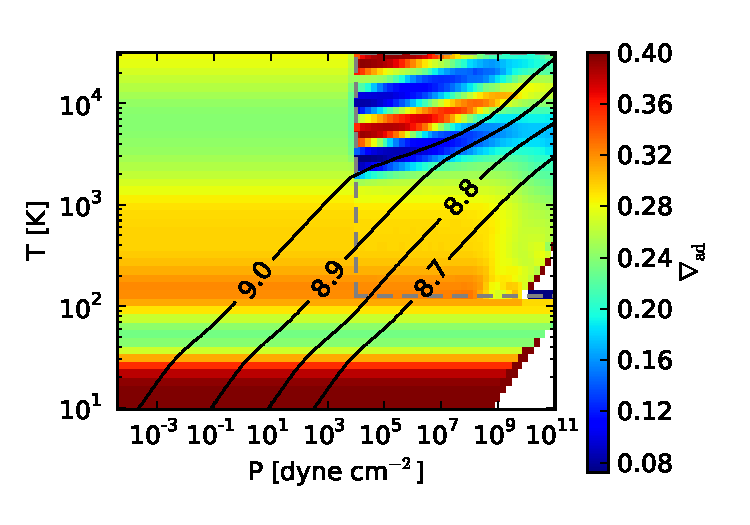
\includegraphics[width=0.5\textwidth]{../../figs/ModelAtmospheres/RadSelfGravRealEOS/PaperFigs/delad_S_mixt.pdf}
%%\vspace{-0.5in}
\caption{Contour plot of the adiabatic gradient $\delad$ for a hydrogen-helium mixture as a function of gas temperature and pressure. The upper-right rectangle encloses the region described by the original \citet{saumon95} EOS tables, while the rest of the plot is our extension. The black curves represent constant entropy adiabats, with the labels $\log_{10}(S)$ [erg K$^{-1}$ g$^{-1}$]. The regions in which the EOS is either invalid or not computed are masked in white. Our extension is only valid for $T \lesssim 2000$ K, since it does not take into account hydrogen dissociation. We choose $T=1500$ K as a conservative temperature cutoff. \citet{saumon95} do not compute the EOS at very high pressures, since hydrogen is solid or may form a Coulomb lattice in this regime, and thus their EOS treatment is no longer valid. While the boundaries of the region in which the free-energy EOS treatment fails can be determined from fundamental thermodynamic constraints, such calculations are not the object of this work. Instead, we note that less pressure is needed for hydrogen to become solid at lower temperatures, and so we choose as boundary a constant entropy curve ($\log(S)=8.4$) above the region in which the \citet{saumon95} model fails. The expressions derived in \App{EOStables} are sufficient to give good results for the colored regions of the extended map, which fully cover the temperature and pressures ranges required by our models.}
\label{fig:deladmap}
\end{figure}
%but not the white ones. We note, however, that the temperature and pressure ranges required by our models are fully covered by the colored regions, where our expressions are valid

%If follows that the expressions derived in \App{EOStables} cannot be used to extend the original tables in this temperature and pressure regime. 

%At high temperatures, hydrogen dissociates and ionizes, while at low temperatures the rotational states of the hydrogen molecule are only partially excited and it no longer behaves like an ideal diatomic gas.

In what follows we explain the behavior of the adiabatic gradient in the three temperature regimes separately.

\vspace{0.2in}

\textbf{1. Intermediate T: Ideal Gas}

For temperatures less than $\sim$$2000$ K but larger than $\sim$$300$ K, the hydrogen molecule is not energetic enough to dissociate and hydrogen behaves as an ideal diatomic gas. We see this in Fig. \ref{fig:deladmap} for 300 K $\lesssim T \lesssim 3000$ K, where the adiabatic gradient is approximately constant. The helium component of the gas causes a slight increase in the adiabatic index: $\delad \approx 0.3$ in this temperature range rather than 2/7 as is the case for a diatomic gas \footnote{Recall $\delad \equiv \frac{\gamma-1}{\gamma}$ for an ideal gas, with $\gamma$ the adiabatic index: $\gamma=7/5$ for a diatomic gas and 5/3 for a monatomic gas.}.

\vspace{0.2in}

\textbf{2. High T: Dissociation and Ionization of Hydrogen.}

At low temperatures, hydrogen exists in molecular form and has a stable configuration. As the temperature becomes higher than $T \sim 2000-3000$ K, the internal energy of the hydrogen molecule becomes large enough to break the covalent bond between the atoms, and hydrogen starts dissociating. Further energy increase at temperatures of $\sim$$10^4$ K results in electrons being removed from atoms, i.e. hydrogen ionizes. In stellar and giant planet interiors there is little overlap between the two processes: hydrogen is almost entirely dissociated into atoms by the time ionization becomes important. 

We see in Figure \ref{fig:deladmap} that the adiabatic gradient decreases significantly in regions of partial dissociation and partial ionization. This behavior is different than that of a mixture of molecular and atomic hydrogen where $2/7<\delad<2/5$, or a mixture of protons and electrons where $\delad=2/5$. We  explain this in what follows. % where hydrogen is either partially dissociated or partially ionized. 

%For a mixture of molecular and atomic hydrogen, we expect the adiabatic gradient to have an intermediate value between monatomic and diatomic gas, while for a mixture of protons and electrons the adiabatic index is just $2/5$ as for a monatomic ideal gas. However, we notice in Fig. \ref{fig:deladmap} that the adiabatic gradient decreases significantly in the regions where hydrogen is either partially dissociated or partially ionized. We further explain this behavior.

For a mixture of ideal gases, the total internal energy is given by the sum of the internal energies of the individual gases. When a gas dissociates, however, part of the internal energy of the system is used to break down molecules, which reduces the amount of energy available to increase the temperature of the system, thus lowering the adiabatic gradient. The energy required to dissociate depends on the dissociation fraction, which can be determined from the Saha equation (see e.g., \citealt{kippenhahn90}). The dissociation fraction only depends on gas temperature and density, and hence only on the EOS. 

An expression for the adiabatic gradient as a function of the dissociation fraction is presented in \App{deladdiss}. As expected, the adiabatic gradient is $\delad=2/7$ for pure molecular hydrogen and $\delad=2/5$ when hydrogen is fully dissociated, but decreases significantly during partial dissociation and is smallest when half of the gas is dissociated. This is consistent with the behavior we see in Figure \ref{fig:deladmap}. 

%At constant entropy, an increase in pressure results in an increase in the internal energy of the system, which usually causes the temperature to rise significantly. During partial dissociation, however, part of the internal energy is used to remove the electrons from atoms, and therefore there is less energy available to increase the temperature of the system. This behavior of constant entropy curves is seen in Figure \ref{fig:deladmap}. 

The ionization of atomic hydrogen is also dictated by the Saha equation, with the dissociation energy replaced by ionization energy, hence the adiabatic gradient has an analogous behavior, consistent with Fig. \ref{fig:deladmap}.


%We now investigate the effect of the low adiabatic index caused by hydrogen dissociation on the luminosity and cooling time evolution of the atmosphere. The left panel of Figure (x) shows the 

%The resulting luminosity and time evolution are shown in Figure \ref{fig:Ltplotall}. We use again instantaneous atmosphere profiles to explain the differences. Figure \ref{fig:ETrprofall} shows the instantaneous temperature and energy profiles, as well as the location of the Bondi radius for a total fixed mass $M_{\rm{tot}}=11.8 M_{\oplus}$. We see that the spin effect at the outer boundary dictates the location of the radiative zone, and therefore the luminosity behavior, while dissociation deep in the atmosphere dictates the energy behavior. As compared to the polytrope, the real EOS therefore generates a deeper radiative zone with a lower luminosity, due to the lower adiabatic index in the outer regions, as well as an atmosphere with the bulk of its energy concentrated at the bottom, due to the low $\delad$ caused by dissociation. As shown above for the ideal gas polytropes, and remembering that $\Delta t \sim -\Delta E/L$, we see that both effects result in a longer time for the atmosphere to evolve.  


\vspace{0.2in}

\textbf{3. Low T: Hydrogen Rotation and Spin Isomers}

As a diatomic molecule, hydrogen has five degrees of freedom, three associated with translational motion and two associated with rotation. The excitation temperature for rotation is $\Theta_r \approx 85$ K for the hydrogen molecule (e.g., \citealt{kittel}), hence the rotational states are fully excited at room temperature. As the gas temperature becomes comparable to $\Theta_r$, fewer rotational states are excited and rotation entirely ceases as $T \rightarrow 0$. %Here we explore the quantum mechanical effects associated with rotation. %We present expressions for the partition function associated with rotation and derive relevant thermodynamic variables in \App{EOStables}. For $T \ll \Theta_r$, the partition function is just equal to one, and no rotational states are excited for very low temperatures and hydrogen behaves like a monatomic gas. On the other hand, if $T \gg \Theta_r$, the molecule is energetic enough for all the rotational states to be fully excited. 

%In this section we discuss the quantum effects of the hydrogen isomeric forms and the way they affect the rotational energy and heat capacity of the hydrogen molecule at low temperatures, and hence the adiabatic gradient. 

 Molecular hydrogen occurs in two isomeric forms, parahydrogen and orthohydrogen. Parahydrogen has antiparallel proton spins and thus an antisymmetric wave function. From the Pauli exclusion principle it follows that it can only occupy symmetric rotational states with even angular quantum number $j$ \citep{farkas35}. In contrast, orthohydrogen has parallel proton spins and a symmetric wave function, and can therefore only occupy states with odd $j$. At equilibrium, the relative abundance of the ortho- and para- states is given by the ratio of their partition functions, described in \App{EOStables}. At $T \rightarrow 0$ all hydrogen molecules are in the ground state with $j=0$, which corresponds to parahydrogen.  As the temperature increases, parahydrogen starts converting into orthohydrogen, resulting in an ortho-para equilibrium ratio of 3:1 at room temperature.
 

The adiabatic gradient scales as $\delad \sim 1/c_{\rm v}=1/(c_{\rm v,t}+c_{\rm v,r}) \sim 1/c_{\rm v, r}$, with $c_{\rm v}$ the specific heat capacity at constant volume, and $c_{\rm v, t}$ and $c_{\rm v,r}$ the translational and rotational components, respectively. The second equality is due to the fact that $c_{v, t}$ is independent of temperature and equal to $3\mathcal{R}/2$. We can therefore understand the $\delad$ behavior by studying the dependence on temperature of $c_{\rm v, r}$ of the ortho-para mixture. 

The internal energy per unit mass and specific heat capacity associated with rotation for the individual isomers and for the equilibrium mixture can be derived from their partition functions (see \App{EOStables} for details), and are plotted in Figure  \ref{fig:ucvr} (after \citealt{farkas35}, Figure 1). At low temperatures, parahydrogen is in the $j=0$ state and has no rotational energy, while orthohydrogen is in the $j=1$ state and has the energy of its first rotational level. Both para- and orthohydrogen, as well as their equilibrium mixture, behave like monatomic gases at low temperatures and thus have zero rotational heat capacity. This is consistent with $\delad=2/5$ at low temperatures as seen in Figure \ref{fig:deladmap}. As the temperature increases, the energetically higher-lying rotational states of para- and orthohydrogen are populated and the heat capacity of both spin isomers increases as a result. We note that the heat capacity of the equilibrium mixture is not a weighted average of the heat capacities of the individual components because it takes into account both the rotational energy uptake of para- and orthohydrogen, and also the shift in their equilibrium concentrations with temperature. This results in a peak in the heat capacity of the mixture around $\sim$$50$ K, as seen in the bottom plot of Figure \ref{fig:ucvr}. As $\delad \sim 1/c_{\rm{v,r}}$, it follows that the adiabatic gradient has to reduce, reach a minimum, then increase as the temperature rises, as shown in Figure \ref{fig:deladmap}.

% As the temperature increases, the energetically higher-lying ($j=1$) ortho-hydrogen is formed, and the concomitant energy increase is seen as a peak in the heat capacity of the equilibrium mixture. 


%There are two significant maxima in the heat capacities of parahydrogen and of the mixture. At very low temperatures, the heat capacity of parahydrogen is zero because only the lowest accessible energy level $j=0$ is occupied and a temperature increase does not provide enough energy to populate the next higher level. When the temperature becomes sufficiently high to populate the second lowest level $j=2$, the heat capacity rapidly increases, passes through a maximum and starts to decrease when the second lowest level becomes saturated. 


%the adiabatic gradient is inversely proportional to the heat capacity, it 

%means that  the former has to first decrease from 2/5 as the temperature increases, reach a minimum around 50 K ($\delad \approx 0.25$ from Fig. \ref{fig:deladmap}), then gradually increase to 2/7 as for a diatomic gas. This behavior is illustrated in Figure \ref{fig:deladmap}.  



%The maxima in the ortho-para mixture appears when parahydrogen starts converting into orthohydrogen. The heat capacity of the equilibrium mixture is not a weighted average of the heat capacities of the individual components because it takes into account both the rotational energy uptake of para- and orthohydrogen, and also the shift in their equilibrium concentrations with temperature. At $T=0$, only parahydrogen is present in the equilibrium mixture; as the temperature is increased, the energetically higher-lying ($j=1$) ortho-hydrogen is formed, and the concomitant energy increase is seen as a peak in the heat capacity. As the adiabatic gradient is inversely proportional to the heat capacity, it means that  the former has to first decrease from 2/5 as the temperature increases, reach a minimum around 50 K ($\delad \approx 0.25$ from Fig. \ref{fig:deladmap}), then gradually increase to 2/7 as for a diatomic gas. This behavior is illustrated in Figure \ref{fig:deladmap}.  



\begin{figure}[h]
\centering
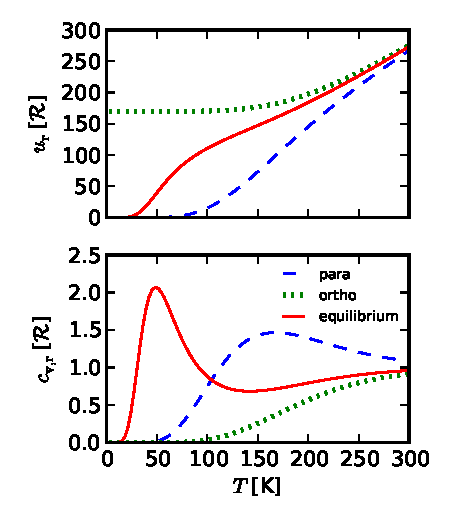
\includegraphics[width=0.5\textwidth]{../../figs/ModelAtmospheres/RadSelfGravRealEOS/PaperFigs/ortho_para_energy.pdf}
%%\vspace{-0.5in}
\caption{Internal energy per unit mass and specific heat capacity associated with rotation for parahydrogen (dashed blue), orthohydrogen (dotted green), and the equilibrium mixture (solids red) as a function of temperature. After \citet{farkas35}, Figure 1.}
\label{fig:ucvr}
\end{figure}

 
 %The partition functions for ortho- and parahydrogen are described in \App{EOStables}.
 %At equilibrium, the relative abundance of the ortho and para states is given by the ratio of their partition functions. For very low temperatures there is only parahydrogen, as molecules are in the ground state with $j=0$, which corresponds to the para state. As the temperature is increased, parahydrogen starts converting into orthohydrogen, resulting in an ortho-para equilibrium ratio of 3:1 at room temperature.

 
  %orthohydrogen, with parallel proton spins, and parahydrogen, with antiparallel proton spins. 
 
 %The Pauli exclusion principle requires the total wavefunction of two fermions, such as protons, to be antisymmetric. As such, a symmetric spin wavefunction requires an antisymmetric rotational wavefunction, and vice-versa (\citealt{farkas35}). Parahydrogen has an antisymmetric spin wavefunction, which means that it can only occupy symmetric rotational states and hence the angular quantum number $j$ has to be even. By analogy, orthohydrogen must have an antisymmetric rotational wavefunction and can only occupy states with odd $j$. The partition functions for ortho- and parahydrogen are described in \App{EOStables}.
 %At equilibrium, the relative abundance of the ortho and para states is given by the ratio of their partition functions. For very low temperatures there is only parahydrogen, as molecules are in the ground state with $j=0$, which corresponds to the para state. As the temperature is increased, parahydrogen starts converting into orthohydrogen, resulting in an ortho-para equilibrium ratio of 3:1 at room temperature.

%\begin{figure}[h]
%\centering
%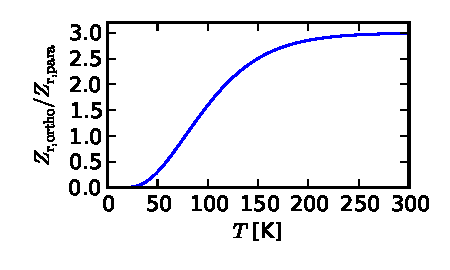
\includegraphics[width=0.5\textwidth]{../../figs/ModelAtmospheres/RadSelfGravRealEOS/EOSeffects/ortho_para_ratio.pdf}
%%%\vspace{-0.5in}
%\caption{Relative abundance of ortho- and parahydrogen as a function of temperature.}
%\label{fig:Zrel}
%\end{figure}

%\vspace{0.1in}

\section{Equation of State Effects on Atmosphere Evolution}
\label{EOSeffects}

Variations in the adiabatic gradient $\delad$ due to partial dissociation and quantum rotational effects (see section \S\ref{deladtable}) have two competing effects on the evolution of a core's atmosphere: (1) they yield a lower envelope luminosity, and (2) a larger amount of energy that needs to be radiated per unit mass, when compared to an ideal gas. Both effects combined slow down accretion and increase the growth time of the atmosphere, and therefore the crossover time and critical core mass. % (both defined in section \ref{intro}). %In this section we explore the effect of partial dissociation and hydrogen spin isomers (see section \ref{deladtable}) on the atmosphere evolution. %Due to the equation of state described in section \ref{deladtable}, a realistic atmosphere will not have a constant adiabatic gradient $\delad$, as was assumed in PY13. We thus first investigate the differences in atmosphere profiles and evolution for ideal gas polytropes with different adiabatic gradients in section \ref{deladpoly}. We then show how the variable adiabatic gradient affects the time evolution of the atmosphere in section \ref{deladeffect}.


%\subsection{Effect of Adiabatic Gradient on Atmosphere Cooling Time}
%\label{deladeffect}

%In this section we discuss the effect of the variable adiabatic index described in subsection \ref{deladinterp} on the atmosphere cooling time. 

%We now explore the separate effects of hydrogen dissociation at high temperatures and spin isomers at low temperatures. From the adiabatic gradient table shown in Figure \ref{fig:deladmap} we find that $\delad$ has the flattest behavior around $T=500$ K. In this region, the gas behaves like an ideal gas with constant polytropic index $\delad \approx 0.3$, with the shift from diatomic gas caused by the helium in the mixture. We generate three sets of atmosphere profiles. The first one corresponds to an ideal gas of constant adiabatic index $\delad=0.3$. The second one is described by the real EOS for temperatures larger than 500 K and by an ideal gas with $\delad=0.3$ for $T<500$ K. Finally, the third profile consists of an ideal gas polytrope with $\delad=0.3$ for $T>500$ K and a real gas in the low temperature regime. We compare the first two profiles to show the dissociation effects, and the first and third profile to show the effects of ortho- and parahydrogen. 

%We now explore the effects of 

%\subsection{Dissociation and Spin Isomers Effects}
%\label{deladeffect}

%In order to investigate the separate effects of hydrogen dissociation at high temperatures and spin isomers at low temperatures on the atmosphere evolution, we generate 



In order to explain the quantum rotational effects at low temperatures, we make the following thought experiment: we imagine that realistic EOS effects only affect the upper atmosphere where temperatures are low, and that the gas is ideal and polytropic deep in the envelope. Conversely, we study the effects of dissociation at high temperatures by assuming that realistic EOS effects only matter at the bottom of the atmosphere where temperatures are high, and that the gas is polytropic in the outer regions. Figure \ref{fig:tplotall} shows the time evolution of atmospheres forming at 10 AU around cores of mass $M\co=10 M_{\oplus}$ and described by various equations of state, as follows:

\begin{itemize}
\item Dashed curve (1) --- ideal gas polytrope with $\delad=0.3$.
\item Dotted curve (2) --- ideal gas polytrope with $\delad=0.3$ for $T>500$ K and realistic EOS for $T<500$ K.
\item Dash-dotted curve (3) --- ideal gas polytrope with $\delad=0.3$ for $T<500$ and realistic EOS for $T>500$ K.
\item Solid curve (4) --- fully realistic EOS.
\end{itemize}
We choose $T=500$ K as the cutoff temperature because the hydrogen-helium mixture behaves like an ideal gas, with $\delad=0.3$, in this temperature regime (see Figure \ref{fig:deladmap}). As such, the difference in cooling times between curves (1) and (2) shows the quantum rotational effects on the atmosphere evolution, while the difference between curves (1) and (3) accounts for hydrogen dissociation. We see that both dissociation and rotational states have a comparable effect on the atmosphere growth and result in slower cooling. The cooling time is dependent on both the total energy released due to the contraction of the envelope and the luminosity of the atmosphere. We explore the relative influence of these two factors separately.

\begin{figure}[h]
\centering
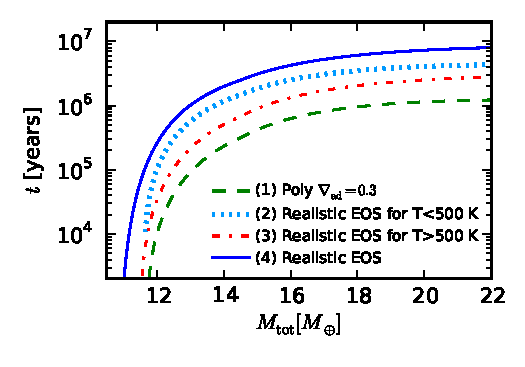
\includegraphics[width=0.5\textwidth]{../../figs/ModelAtmospheres/RadSelfGravRealEOS/PaperFigs/tplot.pdf}
%%\vspace{-0.5in}
\caption{Elapsed time as a function of total mass (core + atmosphere) for a variety of EOS combinations (see text), for a planet forming at 10 AU and with a fixed core mass $M_{\rm c}=10 M_{\oplus}$. Both hydrogen dissociation at high temperatures deep in the atmosphere and quantum rotational effects at low temperatures in the outer envelope result in slower cooling when compared to an ideal gas polytrope.}
\label{fig:tplotall}
\end{figure}

\begin{figure*}[tb]
\centering
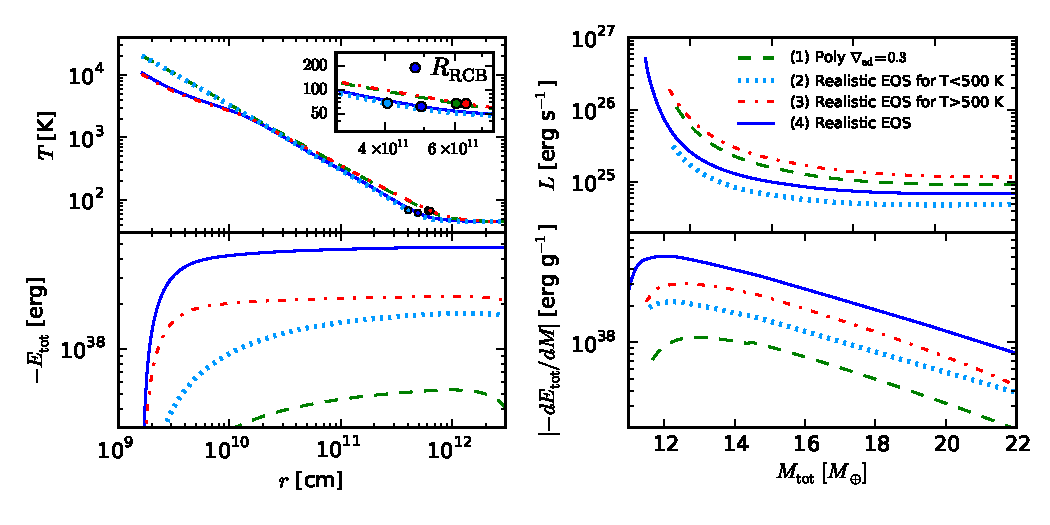
\includegraphics[width=\textwidth]{../../figs/ModelAtmospheres/RadSelfGravRealEOS/PaperFigs/all_plot.pdf}
%%\vspace{-0.5in}
\caption{We explore atmosphere growth around a core of $M\co=10 M_{\oplus}$ forming at 10 AU in our fiducial disk, for the EOS choices in Figure \ref{fig:tplotall}. Upper-left panel:  Instantaneous temperature profile for a total mass (core + atmosphere) of $12 M_{\oplus}$ as a function of radius. The location of the RCB is marked. The quantum rotational effects at low temperatures in the outer region of the atmosphere dictate the location of the RCB. Upper-right panel:  Luminosity evolution as a function of total mass (core + atmosphere). The quantum rotational effects at low temperatures near the top of the atmosphere result in a lower luminosity for the realistic EOS (see text). Lower-left panel: Instantaneous energy profiles as a function on radius for a total mass (core + atmosphere) of $12 M_{\oplus}$. Hydrogen dissociation deep in the atmosphere causes the bulk of the energy to be concentrated at the bottom of the atmosphere. This increases the amount of energy per unit mass that needs to be radiated away, i.e. $|dE/dM|$, resulting in a longer crossover time for the realistic EOS when compared to the polytrope. Lower-right panel:  $|dE/dM|$ evolution as a function of total mass (core + atmosphere). More energy per unit mass has to be radiated away due to hydrogen dissociation when compared to an ideal gas polytrope, which results in slower growth.}
\label{fig:all_plot}
\end{figure*}

The upper-right panel of Figure \ref{fig:all_plot} shows the luminosity evolution with mass for atmospheres (1)-(4), for an example core with $M\co=10 M_{\oplus}$ forming at 10 AU. We see that the lower luminosity of the fully realistic EOS (4) when compared to the polytrope (1) is due to the realistic EOS effects in the outer atmosphere (2). This behavior is directly correlated to the depth of the radiative region of the envelope, which is shown in the upper-left panel of Figure \ref{fig:all_plot} for a total planet mass of $12 M_{\oplus}$. We see that the realistic EOS for low temperatures (2) results in a deeper location of the RCB when compared to the ideal gas polytrope (1). This deeper RCB translates into a larger number of steps that photons need to diffuse to escape from the RCB, and therefore a lower luminosity (cf. equation \ref{eq:delrad}). In fact, a simple estimate of the luminosity emerging at the RCB can be found as follows. 

The equation of radiative diffusion (\ref{eq:structc}) can be approximated in terms of the radiative flux $\mathcal{F}$ as 

\begin{equation}
\label{eq:sigmatau4}
\mathcal{F} \sim \frac{\sigma T\cb^4}{\tau},
\end{equation}
where $\tau$ is the optical depth of the upper radiative layer. Furthermore, we find that $\tau$ is dominated by the optical depth of the first scale height, i.e. 

\begin{equation}
\label{eq:taucb}
\tau \sim \tau\cb=\kappa\cb \rho\cb H\cb,
\end{equation}
where 
\begin{equation}
\label{eq:Hcb}
H\cb=\frac{k_b T\cb}{\mu m_H} \frac{R\cb^2}{G M\cb},
\end{equation}
with $\mu$ the mean molecular weight of the gas, $m_H$ the proton mass, and all other quantities evaluated at the bottom of the radiative layer. By substituting equations (\ref{eq:Hcb}) and (\ref{eq:taucb}) into equation (\ref{eq:sigmatau4}), and noting that $\mathcal{F}=L/(4 \pi (R\cb+H\cb)^2) \approx L / (4 \pi R\cb^2)$, we recover equation (\ref{eq:delrad}) applied at the boundary between the uppermost convective region of the atmosphere and the outer radiative layer (where $\delrad=\delad$).


%We found that the RCB for the fully realistic EOS (4) is roughly at the same location as the RCB for the realistic EOS at low temperatures (2) for low atmosphere masses, and it moves further out relatively as the atmosphere mass increases. This explains our choice of $M_{\rm tot}=12 M_{\oplus}$ as a representative case to illustrate the effect of spin isomers. Envelope growth is slowest at this relative atmosphere-to-core mass (see PY13)... 

Dissociation deep in the planet's atmosphere increases the amount of energy per unit mass that needs to be radiated by the envelope, which further slows down growth. Figure \ref{fig:all_plot}, lower-left plot, shows the total energy (internal and gravitational) profile as a function of the radial coordinate, for the same example planet. The bulk of the energy is concentrated deep in the atmosphere for the realistic EOS at high temperatures (3) and the fully realistic EOS curve (4), which shows that hydrogen dissociation in the inner atmosphere dictates the energy behavior of the envelope. In contrast, energy is concentrated towards the outer boundary for the $\delad=0.3$ polytrope (1). Qualitatively, this can be explained through a simple analytic argument: the density profile in an adiabatic, non-self gravitating atmosphere composed of an ideal gas scales as $\rho(r) \sim r^{1/\delad-1}$ (see also Paper I). Since the energy per unit mass scales as $e(r) \sim \rho(r) r^2 \sim r^{1/\delad+1}$, it is easy to see that adiabats with lower adiabatic gradient have their energy more tightly packed towards the interior of the envelope, which is the case during dissociation when $\delad$ decreases significantly (see section \S\ref{deladtable} and Figure \ref{fig:deladmap}).  It takes more energy to bring in gas deep in the atmosphere for an envelope that has the bulk of its energy concentrated towards the bottom,  which increases the amount of energy per unit mass that needs to be radiated, i.e. $|dE/dM|$, and therefore the cooling time, for the realistic EOS at high temperatures (3) when compared to the ideal gas polytrope (1). This increase in $|dE/dM|$ is shown in the bottom-right panel of Figure \ref{fig:all_plot}.

We have seen that the quantum rotational effect at the outer boundary dictates the location of the radiative zone, and therefore the luminosity behavior, while dissociation deep in the atmosphere dictates the total energy behavior. Overall, both effects result in a longer time for the atmosphere to evolve. 

%we find that only polytropes with $\gamma<3/2$, i.e. $\delad<1/3$, have the total energy concentrated towards the core. This is satisfied by $\delad=2/7$ but not by $\delad=2/5$, in agreement with the results in the bottom panel of Figure \ref{fig:ETrplotpoly}. 
%
%Similarly to section \ref{deladpoly}, we use instantaneous atmosphere profiles to explain the differences. The left panel of Figure \ref{fig:TLrplot} shows the instantaneous temperature profile and the location of the radiative-convective boundary for a total fixed mass (core + atmosphere) $M_{\rm{tot}}=11.8 M_{\oplus}$. The realistic equation of state for low temperatures is characterized by a lower adiabatic index in the outer regions, due to the spin effects, and is therefore dominant in the radiative zone. As a result, it generates a deeper radiative zone with a lower luminosity, which explains the results in the left panel of Figure \ref{fig:TLrplot}. Moreover, since the cooling time is inversely proportional to the luminosity, the spin effect will result in a longer cooling time.
%
%The energy behavior is shown in Figure \ref{fig:Erplot}. The realistic EOS for high temperatures has a low adiabatic index deep in the atmosphere, due to hydrogen dissociation, and thus the bulk of its energy concentrated at the bottom of the atmosphere, for the reasons described in section \ref{deladpoly}. It takes more energy to add mass more mass deep in the atmosphere, and $|dE/dM|$ is larger as a result. 
%%
%
%We have seen that the spin effect at the outer boundary dictates the location of the radiative zone, and therefore the luminosity behavior, while dissociation deep in the atmosphere dictates the energy behavior. Overall, both effects result in a longer time for the atmosphere to evolve. 
%
%\subsection{Ideal Gas Polytropes with Different Adiabatic Gradient}
%\label{deladpoly}
%
%In this section we investigate the differences in luminosity and $dE/dM$, and the resulting time evolution, between ideal gas polytropes with different adiabatic gradients: $\delad=2/7$ (diatomic gas) and $\delad=2/5$ (monatomic gas). We assume both gases have the same mean molecular weight. %We use these results to explain the separate effects of dissociation and spin on the time evolution of the atmosphere.
%
%We generate atmosphere profiles for the two different adiabatic indices at $a=10$ AU and for a core mass $M_{\rm c}=10 M_{\oplus}$, and estimate the luminosity and cooling time evolution as described in section \ref{sec2}. The results are shown in Figure \ref{fig:Ltplotpoly}. We find that the polytrope with the lower adiabatic gradient has both a higher luminosity and a longer cooling time. We use instantaneous atmosphere profiles to explain these effects. 
%
%%We first discuss the effect of the variable adiabatic gradient on luminosity. 
%
%Figure \ref{fig:ETrplotpoly}, top panel, shows the temperature profile for the two polytropes at a fixed total mass $M_{\rm{tot}}=15 M_{\oplus}$. The polytrope with a larger adiabatic gradient, $\delad=2/5$, has a more shallow convective zone, and hence a deeper radiative region, since a larger temperature gradient delays the onset of convection. A deeper radiative layer increases the number of steps that photons need to diffuse, resulting in a lower luminosity as seen in the top panel of Figure \ref{fig:Ltplotpoly}. 
%
%\begin{figure}[h]
%\centering
%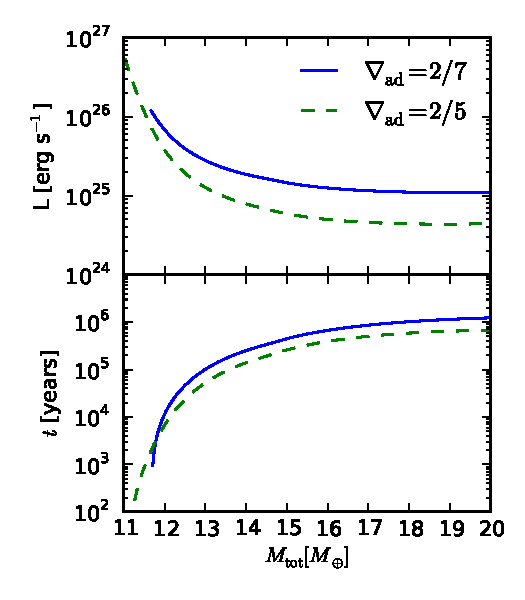
\includegraphics[width=0.5\textwidth]{../../figs/ModelAtmospheres/RadSelfGravRealEOS/PaperFigs/Ltplot_poly.pdf}
%%%\vspace{-0.5in}
%\caption{Luminosity and time evolution as a function of total mass (core + atmosphere) for polytropes with different adiabatic indices, for a planet forming at 10 AU and with a fixed core mass $M_{\rm c}=10 M_{\oplus}$. A larger adiabatic index results in both a lower luminosity and a shorter cooling time.}
%\label{fig:Ltplotpoly}
%\end{figure}
%
%\begin{figure}[h]
%\centering
%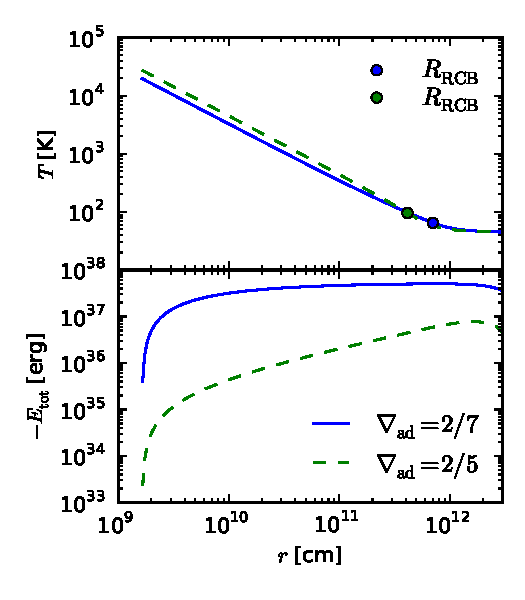
\includegraphics[width=0.5\textwidth]{../../figs/ModelAtmospheres/RadSelfGravRealEOS/PaperFigs/TErplot_poly.pdf}
%%%\vspace{-0.5in}
%\caption{Instantaneous temperature and total energy profiles as a function of radius for polytropes with different adiabatic indices, for a planet forming at 10 AU and with a fixed core mass $M_{\rm c}=10 M_{\oplus}$. The total mass (core + atmosphere) is $15 M_{\oplus}$. The location of the radiative-convective boundary is marked. A lower adiabatic gradient results in a more shallow radiative region (upper panel), and in the total energy being concentrated at the bottom of the atmosphere (lower panel).}
%\label{fig:ETrplotpoly}
%\end{figure}
%
%%In spite of the low luminosity of the atmosphere with $\delad=2/5$, the envelope still grows faster than in the case of a diatomic gas, as shown in the bottom panel of Figure \ref{fig:Ltplotpoly}. This is due to fact that the amount of energy per unit mass that needs to be radiated away, i.e. $|dE/dM|$, is lower for the $\delad=2/5$ polytrope. We have shown in PY13 that polytropes with $\delad=2/7$ have most of the energy concentrated at the bottom of the atmosphere, while polytropes with $\delad=2/5$ have the bulk of the energy towards the outer boundary. 
%
%
%The bottom panel of Figure \ref{fig:ETrplotpoly} shows an instantaneous energy profile for the same total mass $M_{\rm{tot}} = 15 M_{\oplus}$.  The bulk of the energy is concentrated deep in the atmosphere for the $\delad=2/7$ polytrope and towards the outer boundary for the $\delad=2/5$ polytrope. Qualitatively, this can be explained through a simple analytic argument: the density profile in an adiabatic, non-self gravitating atmosphere composed of an ideal gas scales as $\rho(r) \sim r^{1/(\gamma-1)}$ with $\gamma$ the adiabatic index (see PY13). Since the energy per unit mass scales as $e(r) \sim \rho(r) r^2$, we find that only polytropes with $\gamma<3/2$, i.e. $\delad<1/3$, have the total energy concentrated towards the core. This is satisfied by $\delad=2/7$ but not by $\delad=2/5$, in agreement with the results in the bottom panel of Figure \ref{fig:ETrplotpoly}.  It takes more energy to bring in gas deep in the atmosphere for an envelope that has the bulk of its energy concentrated towards the bottom,  which increases $|dE/dM|$ for the $\delad=2/7$ polytrope. 
%
%We find that the energy effect prevails over the luminosity effect, resulting in a longer cooling time for the polytrope with the lower adiabatic gradient (i.e., $\delad=2/7$), as shown in the bottom panel of Figure \ref{fig:Ltplotpoly}.


%From the adiabatic gradient table shown in Figure \ref{fig:deladmap} we find that $\delad$ has the flattest behavior around $T=500$ K. In this region, the gas behaves like an ideal gas with constant polytropic index $\delad \approx 0.3$, with the shift from diatomic gas caused by the helium in the mixture. We generate three sets of atmosphere profiles. The first one corresponds to an ideal gas of constant adiabatic index $\delad=0.3$. The second one is described by the real EOS for temperatures larger than 500 K and by an ideal gas with $\delad=0.3$ for $T<500$ K. Finally, the third profile consists of an ideal gas polytrope with $\delad=0.3$ for $T>500$ K and a real gas in the low temperature regime. We compare the first two profiles to show the dissociation effects, and the first and third profile to show the effects of ortho- and parahydrogen. The resulting time evolution is shown in Figure \ref{fig:Ltplotall}. We see that both dissociation and spin isomers have a comparable effect on the atmosphere growth, and result in slower cooling, and therefore a longer crossover time, when compared to the polytropic ideal gas equation of state. In what follows we explore the two effects separately.




%As compared to the polytrope, the real EOS therefore generates a deeper radiative zone with a lower luminosity, due to the lower adiabatic index in the outer regions, as well as an atmosphere with the bulk of its energy concentrated at the bottom, due to the low $\delad$ caused by dissociation. As shown above for the ideal gas polytropes, and remembering that $\Delta t \sim -\Delta E/L$, we see that both effects result in a longer time for the atmosphere to evolve.  


 



% for an atmosphere described by an ideal gas EOS with $\delad=0.3$ (dashed curve), an atmosphere composed of an ideal gas with $\delad=0.3$ for $T>500$ K and a realistic gas 

%In this section we use the results obtained in section \ref{deladpoly} to explain the effects on the atmosphere evolution of a realistic equation of state. We explore the effect of hydrogen dissociation at the high temperatures in the inner part of the atmosphere, and the effect of hydrogen spin isomers at the low temperatures at the top of the atmosphere separately. In order to do this, we generate atmosphere profiles in which the nebular gas is assumed to be described by a combination of ideal and realistic equations of state, depending on the temperature. To explain the effects of the hydrogen spin isomers in the outer parts of the atmosphere, we assume that the realistic EOS effects only matter at low temperatures; conversely, we assume that the realistic EOS effects are important only at high temperatures in order to study the effects of hydrogen dissociation deep in the atmosphere. As such, we generate three sets of atmosphere profiles, choosing $a=10$ AU and $M\co=5 M_{\oplus}$. The first one is described by a realistic EOS for temperatures larger than 500 K and by an ideal gas with $\delad=0.3$ for $T<500$ K. The second profile consists of an ideal gas polytrope with $\delad=0.3$ for $T>500$ K and a realistic gas in the low temperature regime. Finally, the last profile corresponds to an ideal gas with $\delad=0.3$, the adiabatic gradient of an ideal hydrogen-helium mixture.  We choose $T=500$ K as the reference temperature since the adiabatic gradient of the realistic gas is roughly constant around this temperature (see Figure \ref{fig:deladmap}). The differences in atmosphere structure and evolution between the ideal gas and the realistic gas at low (high) temperatures highlight the effects of hydrogen spin isomers (hydrogen dissociation). Figure \ref{fig:tplotall} illustrates the differences in time evolution between these profiles. We see that both dissociation and spin isomers have a comparable effect on the atmosphere growth, and result in slower cooling, and therefore a longer crossover time, when compared to the polytropic ideal gas equation of state. The cooling time is dependent on both the total energy released due to the contraction of the envelope and the luminosity of the atmosphere. In what follows we explore the relative influence of these two factors separately.


%The resulting time evolution is shown in Figure \ref{fig:tplotall}. We see that both dissociation and spin isomers have a comparable effect on the atmosphere growth, and result in slower cooling, and therefore a longer crossover time, when compared to the polytropic ideal gas equation of state. The cooling time is dependent on both the total energy released due to the contraction of the envelope and the luminosity of the atmosphere. In what follows we explore the relative influence of these two factors separately.

%We now discuss the differences in luminosity and $dE/dM$ between an ideal gas with constant adiabatic gradient and atmospheres with variations in $\delad$ as prescribed by the equation of state discussed in section \ref{EOSeffects}. In what follows we describe our choices of equation of state combinations. From the adiabatic gradient table shown in Figure \ref{fig:deladmap} we find that $\delad$ has the flattest behavior around $T=500$ K. In this region, the gas behaves like an ideal gas with constant polytropic index $\delad \approx 0.3$, with the shift from diatomic gas caused by the helium in the mixture. We generate three sets of atmosphere profiles. The first one corresponds to an ideal gas of constant adiabatic index $\delad=0.3$. The second one is described by the realistic EOS for temperatures larger than 500 K and by an ideal gas with $\delad=0.3$ for $T<500$ K. Finally, the third profile consists of an ideal gas polytrope with $\delad=0.3$ for $T>500$ K and a realistic gas in the low temperature regime. We compare the first two profiles to show the dissociation effects, and the first and third profile to show the effects of ortho- and parahydrogen. The resulting time evolution is shown in Figure \ref{fig:tplotall}. We see that both dissociation and spin isomers have a comparable effect on the atmosphere growth, and result in slower cooling, and therefore a longer crossover time, when compared to the polytropic ideal gas equation of state. The cooling time is dependent on both the total energy released due to the contraction of the envelope and the luminosity of the atmosphere. In what follows we explore the relative influence of these two factors separately.

%We now investigate the effect of the low adiabatic index caused by hydrogen dissociation, on the one hand, and spin isomers on the other hand, on the luminosity and cooling time evolution of the atmosphere, in light of the discussion in section \ref{deladpoly}. The left panel of Figure (x) shows the luminosity evolution with mass for the four combinations of equations of state described in section  

%
%
%\begin{figure}[h]
%\centering
%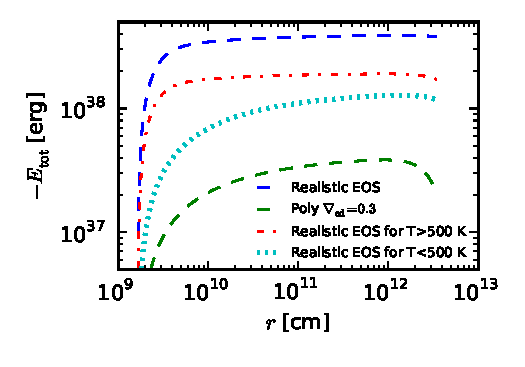
\includegraphics[width=0.5\textwidth]{../../figs/ModelAtmospheres/RadSelfGravRealEOS/PaperFigs/Er_plot.pdf}
%%%\vspace{-0.5in}
%\caption{Instantaneous energy profiles as a function on radius for a variety of EOS combinations, for a planet forming at 10 AU and with a fixed core mass $M_{\rm c}=10 M_{\oplus}$. The total mass (core + atmosphere) is $11.8 M_{\oplus}$. Hydrogen dissociation deep in the atmospheres causes the bulk of the energy to be concentrated at the bottom of the atmosphere. This increases the amount of energy per unit mass that needs to be radiated away, i.e. $|dE/dM|$, resulting in a longer crossover time for the realistic EOS when compared to the polytrope.}
%\label{fig:Erplot}
%\end{figure}





%\subsection{Outer Boundary Effects}

%\textbf{Reemphasize the fact that the atmosphere structure is determined by your outer boundary conditions: T_{out}, P_{out}, R_{out} $\rightarrow$ explore the separate effects of pressure, temperature and a (since the Hill radius is determined by a); show how temperature is the strongest effect. }

\section{Critical Core Mass}
\label{critical}

%\textbf{Define what it is (refer again to paper I also); show the Mcrit vs a for fixed disk life plot, for both real EOS, gamma 7/5 and gamma 5/3; justify the differences in terms of the EOS effects from 4.2; show that using a real EOS makes a significant difference to the results; however, the core masses we get are still doable. Again, a lot of text below will be used but needs reorganizing/rephrasing.}

%\textbf{Define what it is (also refer to paper I) and emphasize how it's different from $M_{crit}$ in standard calculations. Define the crossover mass and crossover time.}


In this section we put together the results obtained in section \S\ref{EOSeffects} and determine the minimum core mass to initiate runaway gas accretion during the lifetime of the protoplanetary disk. As in Paper I, we define this minimum core mass as the \textit{critical core mass}, and the time elapsed until runaway gas accretion is initiated when $M_{\rm{atm}} \sim M\co$ as the \textit{crossover time}. We first explore the dependence of the crossover time on the core mass for a fixed semi-major axis. We then determine the critical core mass to form a giant planet from a gas composed of a realistic hydrogen-helium mixture, and we compare this with the results from Paper I for an ideal diatomic gas. Finally, we determine the critical core mass under more realistic opacity assumptions.

%\subsection{Crossover Time as a Function of Core Mass}
%\label{tvsM}

%\textbf{t vs. M at fixed distance, similar to the plot from paper I. Compare scalings.}

Figure \ref{fig:tvsMplot} displays the time evolution and the crossover time for atmospheres forming around cores with masses between 10 $M_{\oplus}$ and 20 $M_{\oplus}$ at $a=10$ AU in our fiducial disk. The crossover time is shorter for higher mass cores, consistent with the results of Paper I. 

\begin{figure}[h!]
\centering
\includegraphics[width=0.5\textwidth]{../../figs/ModelAtmospheres/RadSelfGravRealEOS/PaperFigs/tco_vs_Matm_10au.pdf}
%%\vspace{-0.5in}
\caption{Elapsed time as a function of atmosphere mass, for cores with fixed masses between $10 M_{\oplus}$ and $20 M_{\oplus}$ at $a=10$ AU in our fiducial disk. The circles mark the crossover time where $M_{\rm{atm}} \sim M_{\rm c}$. The numbers are labeling the core mass in Earth masses. A larger core mass results in a shorter crossover time.}
\label{fig:tvsMplot}
\end{figure}

%\subsection{Critical Core Mass}
%\label{Mcrit}

%\textbf{Mcrit vs. a plot, realistic EOS and polytrope. Discuss the larger critical core mass for the real EOS in light of the effects from section 4.}

Figure \ref{fig:Mvsaplot} shows the critical core mass for a massive atmosphere to form during a typical lifetime of a protoplanetary disk $t=3$ Myrs (e.g., \citealt{jay99}), for a gas described by a realistic EOS and an ISM dust opacity given by equation \ref{eq:opacitylaw}. The results of Paper I for an ideal diatomic gas are plotted for comparison. The inclusion of realistic EOS effects results in a critical core mass more than twice as large than under the ideal gas assumption. As such, non-ideal effects substantially affect the core mass needed to form a giant planet  before the dissipation of the protoplanetary disk.   

\begin{figure}[h!]
\centering
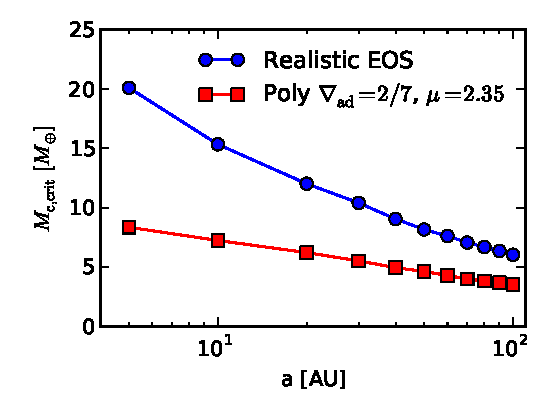
\includegraphics[width=0.5\textwidth]{../../figs/ModelAtmospheres/RadSelfGravRealEOS/PaperFigs/Mc_vs_a_poly_real_paper.pdf}
%%\vspace{-0.5in}
\caption{The minimum core mass for an atmosphere to initiate runaway gas accretion within the lifetime of a typical protoplanetary disk $t \sim 3$ Myrs as a function of semi-major axis, for a realistic hydrogen-helium mixture and a standard ISM power-law opacity. The results of Paper I for an ideal diatomic gas are plotted for comparison. The realistic equation of state yields core masses larger by more than a factor of 2 when compared to the polytrope.}
\label{fig:Mvsaplot}
\end{figure}

The results above were obtained under the assumption that the dust opacity in the radiative region of the atmosphere is given by the standard ISM opacity (see also section \S\ref{struct}). However, our scenario of low planetesimal accretion is likely to favor lower dust opacities, due to grain growth and dust settling. Grain growth, in particular, lowers the absolute value of the opacity and changes the particle size distribution when compared to the standard ISM size distribution (e.g., \citealt{pollack85}). \textbf{Didn't understand comment...}

%Observations of dust in protoplanetary disks (e.g., \citealt{beckwith90}, \citealt{beckwith91}, \citealt{perez12}) have shown evidence for grain growth and that the particle size distribution is not interstellar. 

Although grain growth and evidence for non-ISM size distribution have been observed in protoplanetary disks (e.g., \citealt{beckwith90}, \citealt{beckwith91}, \citealt{perez12}), the size distribution of dust particles has not been tightly constrained. Typically, the grain size distribution is assumed to be a power law: 

\begin{equation}
\label{eq:graindistr}
n \sim a^{-p},
\end{equation}
where $a$ is the particle radius and $p=3.5$ (corresponding to a ``normal'' collisional cascade) or $p=2.5$ (an approximation for coagulation). In this work we use the  \citet{dalessio01} frequency-dependent opacity tables to obtain the temperature-dependent Rosseland mean opacity $\kappa$,  assuming a maximum particle size of 1 cm and a grain size distribution given by equation (\ref{eq:graindistr}) with $p=3.5$ as a fiducial case. Other choices for the power-law coefficient $p$ are discussed later in this section. 

The \citet{dalessio01} opacities are only relevant at temperatures that are sufficiently low for dust grains to remain solid ($T \lesssim 1000$ K). In the temperature regime where dust sublimates we use the \citet{bell94} analytic opacity laws, ensuring smooth transition from the grain growth opacities. 

The sharp drop in opacity ($\kappa \sim T^{-24}$) due to dust sublimation lowers the radiative temperature gradient significantly (see equation \ref{eq:delrad}), and may therefore generate radiative layers within the inner region of the atmosphere (see \App{radwindow}, Figure \ref{fig:delvsr}). This could in principle pose challenges for our model, since the additional luminosity generated in these radiative windows may be large enough to make our assumption of constant luminosity throughout the radiative layers invalid. In practice, however, the inner radiative windows are either very thin (Figure \ref{fig:delvsr}, middle panel), or the temperature gradient is flat enough to result in a roughly constant luminosity throughout the region (Figure \ref{fig:delvsr}, bottom panel; also see equation \ref{eq:structc}). This results in a negligible extra luminosity generated in the radiative windows. While the above is true for our fiducial opacity law, the radiative windows may become non-negligible for other opacity choices and sufficiently low core masses, as we show later in this section. We note that despite the existence of one or more radiative windows in the planet atmosphere, the luminosity that emerges at the outer boundary is set by the top radiative window, as is the case for the standard inner convective-outer radiative envelopes. 

Due to the variable number and position of radiative windows, and therefore radiative-convective boundaries, within the planet atmosphere, we cannot consistently calculate the time evolution of different atmospheres if we evaluate our cooling equation (\ref{eq:coolingglobal}) at the RCB, as we do in our standard model. We choose to evaluate the cooling time at the Bondi radius instead (since our cooling model applies at any radius $R$, see section \S\ref{struct}). We note that our choice of $R$ does not change the estimate of the atmosphere evolution time, to order of magnitude, since the additional luminosity generated in all radiative regions is negligible for our opacity choice (also see Paper I). 

\begin{figure}[h!]
\centering
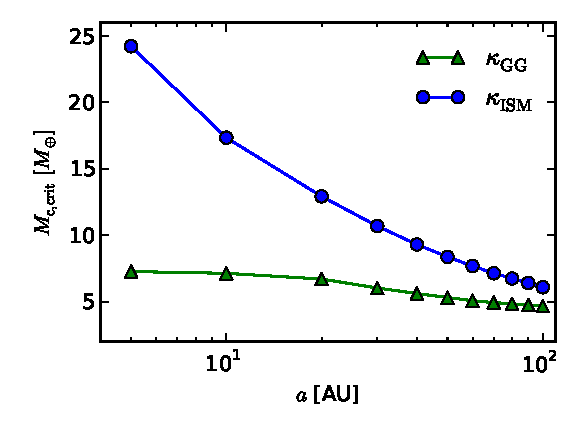
\includegraphics[width=0.5\textwidth]{../../figs/ModelAtmospheres/RadSelfGravRealEOS/PaperFigs/Mcrit_vs_a_gg.pdf}
%%\vspace{-0.5in}
\caption{Critical core mass as a function of semi-major axis for radiative opacities that account for grain growth. The critical core mass is lower than in our fiducial case where dust grains have a standard ISM distribution.}
\label{fig:Mcritvsagg}
\end{figure}

Figure \ref{fig:Mcritvsagg} shows the resulting critical core mass as a function of semi-major axis. The critical core mass is lower than in the standard case, and less sensitive to the distance in the disk, i.e. the boundary conditions (temperature and pressure). We have shown in Paper I that the critical core mass is highly dependent on disk temperature rather than pressure. The temperature dependence, however, is mainly due to opacity: for the simplified analytic model developed in Paper I we found that the crossover time $t_{\rm co} \sim T^{\beta+1/2}$, with $\beta$ the power-law exponent in equation (\ref{eq:opacitylaw}). Opacity is less sensitive to temperature variations for larger grains and has an almost flat profile (see Figure \ref{fig:opacity}), which results in $\beta \ll 1$ and a much weaker temperature (and therefore semi-major axis) dependence of the critical core mass, as seen in Figure \ref{fig:Mcritvsagg}. Moreover, grain growth reduces the absolute value of the opacity, which results in an overall lower crossover time and critical core mass. 

\begin{figure}[h!]
\centering
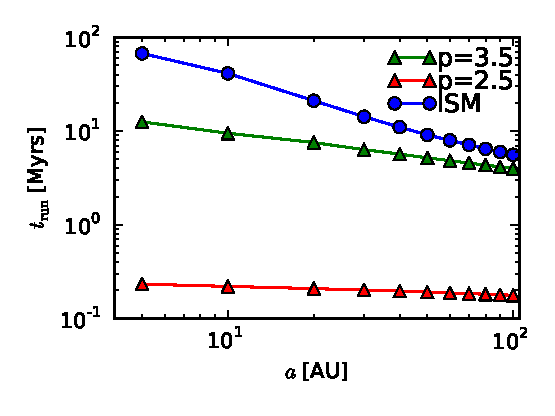
\includegraphics[width=0.5\textwidth]{../../figs/ModelAtmospheres/RadSelfGravRealEOS/PaperFigs/tco_vs_a_Mc4_comp.pdf}
%%\vspace{-0.5in}
\caption{Crossover time for different grain size distribution, for a planet forming around a core $M\co=4 M_{\oplus}$. The standard ISM result is plotted for comparison. The crossover time is more than one order of magnitude lower when coagulation is accounted for, i.e. $p=2.5$.}
\label{fig:p25p35}
\end{figure}

In our calculation so far we assumed that the size distribution of dust grains is the power law (\ref{eq:graindistr}) with $p=3.5$, which corresponds to a normal collisional cascade. If, however, coagulation is taken into account, the exponent $p$ can be approximated as $p=2.5$ \citep{dalessio01}. This results in a flatter and significantly lower opacity, which may substantially reduce the critical core mass. However, we have found that our model breaks down for low core masses ($M_{\rm c} \lesssim 3 M_{\oplus}$) under this assumption, i.e. the outer radiative region becomes deep enough that the luminosity generated in this region can no longer be neglected. Figure \ref{fig:p25p35} shows the crossover time as a function of semi-major axis for the lowest core mass in which our model is valid, $M_{\rm c}=4 M_{\oplus}$. The crossover time is more than one order of magnitude lower when coagulation is accounted for, which implies that the critical core mass may be, in fact, significantly lower than presented in Figure \ref{fig:Mcritvsagg}. 



%\section{Model Relevance in Planet Formation Theory}
\section{Effects of Planetesimal Accretion}
\label{acc}

In this study we have considered protoplanets with fully formed cores for which planetesimal accretion is negligible and KH contraction dominates the luminosity evolution of the atmosphere. This is different from calculations that assume high planetesimal accretion rates and find that the atmosphere is in steady state and solely heated due to accretion of solids. In this section we compare our results for the critical core mass to analogous results from steady-state analytic calculations. We discuss the core accretion rates that are necessary for our regime to be valid in section \S\ref{raf1}. In section \S\ref{raf3}, we estimate core growth during atmosphere evolution at the maximum rate for which the KH regime is valid, and show it is negligible. Finally, we compare our results with those assuming fast planetesimal accretion in section \S\ref{raf2}.

 %In this section we investigate the core accretion rates that are necessary for our regime to be valid. We also discuss the conditions under which runaway gas accretion can be initiated due to the Kelvin-Helmholtz contraction of the atmosphere before it becomes critical due to planetesimal accretion.

\subsection{Planetesimal Accretion Rates}
\label{raf1}

Kelvin-Helmholtz contraction dominates an atmosphere's luminosity if  $L_{\mathrm{acc}} < L_{\rm{KH}}$, where $L_{\rm{acc}}$ is the accretion luminosity,

\begin{equation}
\label{eq:Lacc}
L_{acc}=G \frac{M_{\rm{c}} \dot{M_{\rm{c}}}}{R_{\rm{c}}},
\end{equation}
and $K_{\rm KH}$ is given by equation (\ref{eq:coolingglobal}) with $L\co=\Gamma=0$ (see section \ref{struct}). This condition is satisfied as long as the planetesimal accretion rate 

\begin{equation}
\label{eq:McdotKH}
\dot{M\co}<\dot{M}_{\rm c, KH} \equiv \frac{L_{\rm KH} R\co}{G M\co}.
\end{equation} 

To calculate $\dot{M}_{\rm c, KH}$, we choose as a fiducial case an atmosphere forming at 10 AU and with a core mass of $10 M_{\oplus}$. Since analytic studies assume an ideal gas EOS, for ease of comparison we choose an ideal gas polytrope with constant adiabatic gradient $\delad=2/7$ and mean molecular weight $\mu=2.35$ (see also Paper I). For this choice of parameters, the atmosphere crossover time is $t _{\rm{co}}\sim$ 1.2 Myrs, which is within the typical lifetime of a protoplanetary disk. The results are presented in Figure \ref{fig:accrates}. The atmosphere growth rate $\dot{M}_{\rm{atm}}$ is also plotted for comparison. We see that the core accretion rate has to be $\sim2-3$ orders of magnitude lower than the atmosphere accretion rate for our assumptions to be valid.  If the core had accreted planetesimals at the $\dot{M}_{\rm c, KH}$ rate since it started forming, it couldn't have grown large enough to attract an atmosphere within typical disk lifetime. This is consistent with the requirement of our model that the planetesimal accretion rate is initially large during core growth, then significantly reduces as the gaseous envelope accumulates. This is a plausible scenario, as the core may have formed in the inner part of the disk and was later scattered outwards \citep{ida13}, or the planet's feeding zone could have been depleted of solids due to a giant neighbor.  We further estimate two reference accretion rates. The first one is the core accretion rate $\dot{M}_{\rm c, acc}$ needed to grow the core to $M\co=10 M_{\oplus}$ on the same timescale as our model atmosphere, $\tau=1.2$ Myrs:

\begin{equation}
\label{eq:Mcdot}
\dot{M}_{\rm{c,acc}}(M_{\rm{c}}) \equiv \frac{M_{\rm{c}}}{\tau}.
\end{equation}
The second reference planetesimal accretion rate is $\dot{M}_{\rm c, Hill}$, a typically assumed planetesimal accretion rate for which the random velocities of the planetesimals are of the order of the Hill velocity around the protoplanetary core (for a review, see \citealt{goldreich04}). This is the accretion rate at the boundary between the dispersion dominated and shear dominated regimes. Following \citet{rafikov06} (equation A1),

\begin{equation}
\label{eq:MdotHill}
\dot{M}_{\rm{c,Hill}}=\Omega \Sigma_{\rm p} R\co R_{\rm H},
\end{equation}
where $\Sigma_{\rm p}$ is the surface density of solids, assumed to satisfy $\Sigma\di \approx 100 \Sigma_{\rm p}$ for a dust-to-gas ratio of 0.01.


 \begin{figure}[h]
\centering
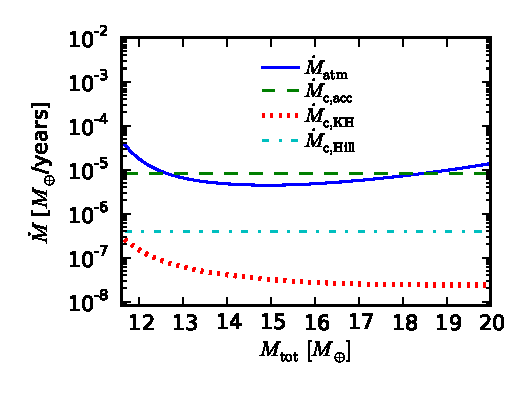
\includegraphics[width=0.5\textwidth]{../../figs/ModelAtmospheres/RadSelfGravRealEOS/PaperFigs/acc_rates_paper.pdf}
%\vspace{-0.5in}
\caption{Various accretion rates in the case of a planet forming at 10 AU and with a core mass $M\co=10 M_{\oplus}$, for a polyropic EOS and ISM power-law opacity. For this choice of parameters, the crossover time (defined in section \S\ref{critical}) is $t_{\rm co} \sim 1.2$ Myrs. The $\dot{M}_{\rm{atm}}$ (solid blue) curve represents the growth rate of the atmosphere as estimated by our model, and $\dot{M}_{\rm{c,KH}}$ (dotted red) is the maximum planetesimal accretion rate during the gas contraction phase in order for our regime to be valid, i.e. $L_{\mathrm{acc}} < L_{\rm{KH}}$ (see text). For comparison, we plot the core accretion rate $\dot{M}_{\rm{c,acc}}$ (dashed green) necessary to grow the core on a timescale $\tau=t_{\rm co}$, and a typically assumed planetesimal accretion rate $\dot{M}_{\rm{c,Hill}}$ (dash-dotted light blue) for which the random velocity of the planetesimals is given by the Hill velocity due to the core (see text). We note that $\dot{M}_{\rm c, KH}$ and $\dot{M}_{\rm c, Hill}$ are both lower than $\dot{M}_{\rm c, acc}$, consistent with our assumptions that planetesimal accretion must have slowed down after core growth.}
\label{fig:accrates}
\end{figure}


\subsection{Core Growth during KH Contraction}
\label{raf3}

In this section we investigate whether planetesimal accretion during the gas contraction phase at the rate $\dot{M}<\dot{M\co}_{\rm{KH}}$  can alter the core mass enough to affect the time evolution of the atmosphere. We can quantitatively estimate the increase in core mass as 

\begin{equation}
\label{eq:cminc}
\Delta M_{\rm{c}} = \int_0^{t_{\rm{co}}} \dot{M_{\rm{c}}} dt \approx \sum_i \dot{M_{\rm{c}}}_i \Delta t_i,
\end{equation}
 
 \noindent where the accretion rate $ \dot{M_{\rm{c}}}_i $ is given by 
 
 \begin{equation}
 \label{eq:Mdotexp}
 \dot{M_{\rm{c}}}_i =\frac{L_i R\co}{G M_{\rm{c}}} 
 \end{equation}
 
 \noindent from equation (\ref{eq:Lacc}), with $L_i$ the luminosity of the atmosphere at time $t_i$ in our model. For $M_{\rm{c}}=10 M_{\oplus}$, we find $\Delta M_{\rm{c}} \approx 0.2 M_{\oplus} \ll 10 M_{\oplus}$. It follows that a significant increase in core mass that could potentially alter the time evolution of the atmosphere would occur on a much longer timescale then the crossover time for the unperturbed atmosphere. The time evolution of the atmosphere is thus insensitive to core mass changes at a rate imposed by the assumption that $L_{\rm{acc}}<L_{\rm{KH}}$.


 %It is easy to see that  $\dot{M}_{\rm{c,typical}}$ is more than one order of magnitude lower than the gas accretion rate of our model atmosphere $\dot{M}_{\rm{atm}}$, and lower than the core accretion rate $\dot{M}_{\rm{c,acc}}$ needed to grow the core and the atmosphere at the same time within the disk life time. As such, the formation of a giant planet by growing the core first, then letting the atmosphere cool is faster than growing the core and the atmosphere at the same time at a steady planetesimal accretion rate.

\subsection{Comparison with Steady-State Results}
\label{raf2}

Next, we check that runaway gas accumulation due to planetesimal accretion cannot already commence before the atmosphere becomes unstable due to KH contraction, as our regime is no longer relevant under such conditions. We recall that in steady-state studies, the critical core mass is  the maximum core mass for which the atmosphere is still in hydrostatic balance; runaway gas accumulation occurs if the core mass grows further. A higher planetesimal accretion rate results in a larger critical core mass for the steady-state models. As such, if unstable atmosphere collapse does not occur due to planetesimal accretion for the lowest value of $\dot{M}_{\rm c, KH}$ over the course of the atmosphere's growth (see, e.g., Figure \ref{fig:accrates}), then it can only occur in the KH dominated regime. In what follows we calculate the critical core mass $M_{\rm crit, KH}$ corresponding to $\min(\dot{M}_{\rm c, KH})$ and show that it is higher that the critical core mass we determined in the KH dominated regime. 

%The maximum planetesimal accretion rate $\dot{M}_{\rm c, KH}$ that satisfies equation (\ref{eq:McdotKH})

%is denoted by the dotted line in Figure \ref{fig:accrates} for $a=60$ AU and $M\co=5M_{\oplus}$. If unstable atmosphere collapse does not occur due to planetesimal accretion for the lowest value of $M_{\rm c, KH}$, then runway gas accretion can only occur in the KH dominated regime. In what follows we calculate the critical core mass $M_{\rm c, KH}$ corresponding to $\dot{M}_{\rm c, KH}$ and show that it is higher than our calculated critical core mass. 

%A core that forms on the same timescale as our model atmosphere accretes planetesimals at a rate given by equation (\ref{eq:Mcdot}). 

%This accretion rate is dependent on the core mass, which is steadily increasing. We therefore compare the critical core mass due to planetesimal accretion at this rate $M_{\rm{crit,acc}}$ to the critical core mass as defined in our estimates $M_{\rm{c,crit}}$ (see section \ref{critical}). If $M_{\rm{crit,acc}}<M{\rm_{c, crit}}$, then the atmosphere has already initiated unstable gas accretion by the time Kelvin-Helmholtz contraction starts dominating. 

%Specifically, we compare the critical core mass due to planetesimal accretion at the rate 

%we compare the critical core mass $M_{\rm{c,acc}}$ due to planetesimal accretion, for an accretion rate that satisfies $L_{\rm{acc}}<L_{\rm{KH}}$ to the actual core mass $M_{\rm{c}}$ assumed fixed in our model. If $M_{\rm{c,acc}}<M{\rm{c}}$, then the atmosphere has already initiated unstable gas accretion by the time Kelvin-Helmholtz contraction starts dominating. 

In order to estimate $M_{\rm crit, KH}$, we use the results of \citet{rafikov06} for low luminosity atmospheres forming in the outer disk ($>2-5$ AU), consistent with our region of interest. \citet{rafikov06} assumes an ideal gas polytropic EOS and a lower opacity than the standard ISM opacity that we use in our calculations (see equation \ref{eq:opacitylaw}). We thus calculate the critical core mass for an ideal gas polytrope with the normalization factor $F_{\kappa}$ reduced by a hundred, which is comparable to the opacity law used by \citet{rafikov06} \footnote{The power-law opacity of \citet{rafikov06} is scaled to the (semi-major axis dependent) disk temperature, while our opacity is scaled to an absolute reference temperature. We thus cannot directly use the \citet{rafikov06} opacities for our comparison.}. %(see Paper I). 

Following \citet{rafikov06}, we find the following expression for the critical core mass when accretion luminosity dominates the evolution of the atmosphere:

\begin{equation}
\label{eq:critraf}
M_{\rm{crit, KH}} \sim \Big[\frac{\min[\dot{M}_{\rm c, KH}(M_{\rm{c}})]}{64 \pi^2 C} \frac{\kappa_0}{\sigma G^3} \frac{1}{R\co M\co^{1/3}} \Big(\frac{k_b}{\mu}\Big)^4\Big]^{3/5},
\end{equation}
with $C$ an order unity constant depending on the adiabatic gradient and disk properties (see \citealt{rafikov06}, equation B3). From equation (\ref{eq:McdotKH}), the accretion rate $\dot{M}_{\rm c, KH}$ depends on the core mass $M\co$. We find $M_{\rm crit, KH}$ numerically by setting $M\co=M_{\rm crit, KH}$ on the right-hand side of equation (\ref{eq:critraf}). The result is displayed in Figure \ref{fig:raf2}; the critical core mass corresponding to planetesimal accretion at the rates displayed in Figure \ref{fig:accrates} is displayed for comparison.  

 \begin{figure}[h]
\centering
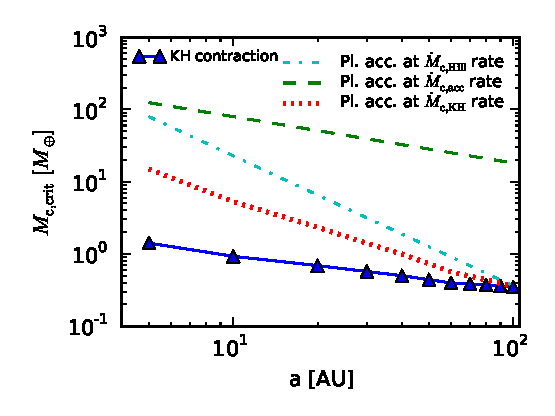
\includegraphics[width=0.5\textwidth]{../../figs/ModelAtmospheres/RadSelfGravRealEOS/PaperFigs/Mc_vs_a_poly_comp.pdf}
%\vspace{-0.5in}
\caption{Comparison between the critical core mass $M_{\rm{crit, KH}}$ due to planetesimal accretion and the assumed fixed core mass when gas contraction dominates. Our results yield lower core masses than in the fast planetesimal accretion case (e.g., \citealt{rafikov06}). The critical core mass corresponding to $\dot{M}_{\rm c, Hill}$ and $\dot{M}_{\rm c, acc}$ from Figure \ref{fig:accrates} is plotted for comparison.}
\label{fig:raf2}
\end{figure}

The critical core mass due to KH contraction is smaller than in the case in which planetesimal accretion dominates the evolution of the atmosphere. This brings us to two conclusions. First, we confirm that planetesimal accretion can be safely ignored in our regime of interest. Secondly, this comparison tells us that the core mass needed to form a giant planet is smaller if the core forms first, then accretes a massive envelope, than in the case where the core and atmosphere grown simultaneously in a high planetesimal accretion regime. Moreover, our result represents a true, absolute minimum on the core mass needed to form a giant planet during the lifetime of the protoplanetary disk, as our core no longer grows.

% \textbf{This works for this particular choice of core, disk etc. conditions, and I am expecting it to work for most of our parameter space, but it would probably be good to explore this numerically, at least to order of magnitude, with the estimates we have.} 

%This means that for large core masses, planetesimal accretion will lead to runaway gas accretion before gas contraction starts dominating, and hence our model is not applicable in that regime. However, we have found in section \ref{critcore} that unstable atmospheres collapse occurs within the life time of the disk for protoplanetary cores smaller than this. 


%\section{Model Validity??? \textbf{(for now, in lack of a better title)}}
%
%\textbf{Discuss geometric effects (spherical symmetry in the inner disk), opacity effects (also in the 	inner disk) and planetesimal accretion; from this build the parameter space where the model is 	valid and confirm from the plots in the previous section that this is where we're looking. Part of the text regarding the planetesimal accretion discussion is below, as initially written for Paper I}
%
%\subsection{Geometric Effects}
%\subsection{Opacity Effects}
%
%
%\section{Discussion}
%\label{discussion}

%In this section we discuss the parameter space of validity of our model. We calculate the conditions under which planetesimal accretion can be ignored, and review the effects of some of the approximations that come into our model.
%
%  
 \section{Conclusions}
 \label{conclusions}
 
 In this paper we study the formation of giant planets embedded in a gas disk. We consider atmosphere evolution around fully grown cores and determine the minimum (critical) core mass required to form a gas giant during the typical lifetime of a protoplanetary disk. We improve the model developed in Paper I (\textbf{does this also need to be written out as Piso \& Youdin?}) by including realistic equation of state (EOS) tables and dust opacities. For a realistic EOS and interstellar grain opacity, the critical core mass is $\sim$$20 M_{\oplus}$ at 5 AU and drops to $\sim$$6 M_{\oplus}$ in our fiducial disk. These results are more than twice as large than those calculated in Paper I for a polytropic EOS, and bring the critical core mass to $\sim$$10 M_{\oplus}$, the value typically quoted in many core accretion studies. When realistic opacities that include grain growth are used, the critical core mass is significantly lower, i.e. $\sim$$6 M_{\oplus}$ at 5 AU and $\sim$$4 M_{\oplus}$ at 100 AU. Different assumptions about the grain size distribution (e.g., that take into account coagulation) may further reduce the critical core mass.
 
Our results yield lower core masses than analogous results that consider high planetesimal accretion rates for which the core and atmosphere grow simultaneously. It is thus possible to form a giant planet from a smaller core if the core grows first, then the accretion rate of solids is reduced and a gaseous envelope is accumulated. Moreover, since additional heat sources such as planetesimal accretion limit the ability of the atmosphere to cool and undergo Kelvin-Helmholtz contraction, our results represent a true minimum on the core mass needed to form a giant planet during the typical lifetime of a protoplanetary disk.
 
  
% In this paper we study giant planet formation assuming that planetesimal accretion is negligible and the atmosphere evolution is dominated by KH gas contraction. We use the model developed in Paper I to determine the critical core mass to form a giant planet before disk dissipation assuming that the nebular gas obeys a realistic EOS that takes into account non-ideal effects. We find that variations in the adiabatic gradient due to thermodynamic effects such as dissociation and hydrogen spin isomers result in a critical core mass more than twice as large than in the case of a gas described by an ideal gas polytrope. This brings the critical core mass to $M_{\rm{c, crit}} \sim 10 M_{\oplus}$, which is the value typically quoted in many core accretion studies (see PY 13). We further make realistic assumptions about the dust opacity in the protoplanetary disk by taking into account grain growth. The resulting critical core mass is much less sensitive to outer boundary conditions (disk temperature and pressure) and is found to be $M_{\rm{c, crit}} \sim 5 M_{\oplus}$. Different grain size distribution assumptions (i.e., that take into account coagulation) may further reduce the critical core mass.
  
 %While for an ideal diatomic gas the minimum core mass to form a giant planet under the assumptions of our model is lower than the typically quoted value of $10 M_{\oplus}$ (see PY13), the inclusion of non-ideal effects brings this values back to around $10 M_{\oplus}$
 
% We also compare our results to studies that assume high planetesimal accretion rates, due to which the atmosphere is in steady state and entirely heated by planetesimals, and find that that our model yields lower critical core masses. This shows that it is easier to form a giant planet by growing the core first, then reducing the planetesimal accretion rate and letting the atmosphere evolve on a KH time scale. Moreover, since additional heat sources such as planetesimal accretion limit the ability of the atmosphere to cool and undergo KH contraction, our results represent a true minimum on the core mass needed to form a giant planet during the typical lifetime of a protoplanetary disk.
 
% In this paper we have studied the formation of giant planet atmospheres under the assumption that Kelvin-Helmoholtz gas contraction dominates the luminosity evolution of the atmosphere over planetesimal accretion. We built quasi-static two-layer atmosphere models with an inner convective region and an outer radiative region that matches smoothly onto the protoplanetary disk. We derived a cooling model to connect series of quasti-static atmospheres, and thus obtained an evolutionary history of the envelope. We defined the time at which unstable atmosphere collapse commences as $M_{\rm atm}(t)\sim M_{\rm c}$. From this we defined as ``critical core mass'' the minimum core mass for a protoplanet to initiate runaway gas accretion during the lifetime of the protoplanetary disk. We studied this minimum mass for a variety of disk conditions, nebular gas compositions and opacities. We found that the critical core mass decreases as we move further out in the disk, and is smaller for lower disk temperatures and opacities and for higher mean molecular weight of the gas. 
% 
% We find that the critical core mass to form a giant planet within the life time of the disk is smaller than the results yielded by studies that assume that the atmosphere evolution is dominated by the luminosity due to planetesimal accretion. We have showed that the planetesimal accretion rate needed to grow the core on a typical disk time scale is larger than the expected planetesimal accretion rates at large separations. As such, it is faster to form a planet by growing the core first in a fast planetesimal accretion regime (e.g., the core forms in the inner disk, then migrates outwards), then significantly reduce planetesimal accretion and allow a massive atmosphere to accumulate. 
 
%Our study assumes that the protoplanetary core forms first, then it r
 
%---------------------------------------------------------------------------
\bibliographystyle{apj}
\bibliography{refs}

\appendix
\section{Equation of State Tables}\label{EOStables}

In this study we consider atmosphere growth in the outer parts of protoplanetary disks ($a \lesssim 100$ AU), where temperature and pressure drop to $T \sim 20$ K and $P \sim10^{-4}$ dyn cm$^{-2}$ for our MMSN disk model (see equations \ref{eq:diskb} and \ref{eq:Pd}). We assume that the nebular gas is described by a realistic equation of state (EOS), as prescribed by the \citet{saumon95} EOS tables. However, these tables only cover a relatively high range of temperatures and pressures, i.e. $2.1 < \log_{10} T(\rm{K})<7.06$ and $4.0<\log_{10}P$(dyn cm$^{-2})<19.0$. We thus need to extend the tables to lower $T$ and $P$, as required by our disk model. We choose $\log_{10} T =1.0$ and $ \log_{10}P=-4.4$ as our lower boundaries for temperature and pressure, respectively, resulting in an extended temperature and pressure grid 

\begin{eqnarray}
1.0 & < & \log_{10} T <2.1, \\ 
-4.4& < & \log_{10} P<4.0. \\
\end{eqnarray} 
The other thermodynamic variables in the tables are calculated as follows.



%In this section we explain the procedure for extending and interpolating the \cite{saumon95} EOS tables. The EOS takes into account non ideal interactions, and includes physical treatments of dissociation and ionization. However, the \cite{saumon95} EOS tables only cover a relatively high range of temperatures and pressures: $2.10 < \log_{10} T(\rm{K})<7.06$ and $4<\log_{10}P$(dyn cm$^{-2})<19$. We consider cold disks, where the temperature and pressure drop to $\sim 20$ K and $\sim 10^{-4}$ dyn cm$^{-2}$, respectively (see equations (\ref{eq:diskb}) and (\ref{eq:Pd})). It is therefore necessary to extend the \cite{saumon95} EOS tables to lower temperature and pressure values.

%We choose $\log_{10} T (\rm{K})=1$ and $ \log_{10}P$(dyn cm$^{-2})=-4.4$ as our lower boundaries for temperature and pressure, respectively. Our temperature and pressure grid becomes: $1 < \log_{10} T(\rm{K})<7.06$ and $-4.4<\log_{10}P$(dyn cm$^{-2})<19$. The other thermodynamic variables in the tables are calculated as follows.

\subsection{Hydrogen}

\label{hydrogen}

For a system of particles, the partition function can be written as the product of all partition functions associated with each type of energy that the system can have:

%\begin{equation}
%\label{eq:z}
%Z=Z_t Z_r Z_v Z_e Z_n,
%\end{equation}

\begin{equation}
\label{eq:zagain}
Z=Z_t Z_r Z_v
\end{equation} 

\noindent where $Z_t$, $Z_r$, $Z_v$ are the partition functions associated with translation, rotation, and vibration, respectively \footnote{We ignore electronic and nuclear excitation as they are only important at temperatures much higher than our regime of interest}. Our derivations follow \citet{kittel} %For hydrogen, electronic and nuclear excitation are only significant at temperatures higher than our region of interest ($\theta_e \approx 12000$ K and $\theta_n >> \theta_e$, where $\theta_e$ and $\theta_n$ are the characteristic temperatures for electronic and nuclear excitation, respectively). As such, we will only take into account the translation, rotation and vibration of the hydrogen molecule:

%In what follows we present and briefly derive expressions for thermodynamic variables based on quantum mechanics principles. More details on the derivations can be found in \citet{kittel}.

In the classical limit, the partition function associated with the motion of the center of mass of a gas molecule of mass $m$ is given by:

\begin{equation}
\label{eq:Zt}
Z_t=(m/2 \beta \pi \hbar^2)^{3/2} V,
\end{equation}
with  $T$ and $V$ the gas temperature and volume, respectively, $\hbar$ the reduced Planck constant, and  $\beta=1/(k_b T)$. The rotational partition function is generally written as:

\begin{equation}
\label{eq:Zr}
Z_r=\sum_0^\infty (2 j+1) \exp{\Big[\frac{-j (j+1)\Theta_r}{T}\Big]},
\end{equation}

\noindent where $\Theta_r$ is the characteristic temperature for rotational motion. In the case of hydrogen, $\Theta_r \approx 85$ K. However, molecular hydrogen occurs in two isomeric forms: orthohydrogen, with the proton spins aligned parallel to each other, and parahydrogen, with the proton spins aligned antiparallel. Parahydrogen can only a have symmetric (even) wave function associated with rotation, while orthohydrogen can only have an antisymmetric (odd) wave function associated with rotation (see section \S\ref{deladtable} for an explanation why). The rotational partition functions for ortho- and parahydrogen can thus be written as:

\begin{equation}
\label{eq:Zpara}
Z_{\rm{r,para}}=\frac{1}{2}\sum_0^\infty (1+(-1)^j) (2 j +1) \exp\Big[-\frac{j(j+1)\Theta_r}{T}\Big]
\end{equation}
and
\begin{equation}
\label{eq:Zortho}
Z_{\rm{r,ortho}}=\frac{3}{2}\sum_0^\infty (1-(-1)^j) (2 j +1) \exp\Big[-\frac{j(j+1)\Theta_r}{T}\Big]
\end{equation}
The factor of 3 above accounts for the three-fold degeneracy of the ortho state.

 When the two isomers are in equilibrium, the combined partition function is given by the sum of the individual partition functions, $Z_{\rm r}=Z_{\rm{r, ortho}}+Z_{\rm{r,para}}$ and can be written as:

\begin{equation}
\label{eq:Zrspin}
Z_r=\sum_0^\infty (2-(-1)^j) (2j+1) \exp{\Big[\frac{-j (j+1) \Theta_r}{T}\Big]}
\end{equation}
In our range of temperatures of interest, we found that $Z_r$ converges after about 25 terms in the series.


Finally, the partition function for vibrational motion is given by:

\begin{equation}
\label{eq:Zv}
Z_v=[1-\exp{(\theta_v/T)}]^{-1},
\end{equation}

\noindent where $\theta_v$ is the characteristic temperature for vibrational motion, $\theta_v \approx 6140$ K for hydrogen. 

If the partition function of a system particles is known in terms of $(V, T)$, the internal energy per unit mass, entropy per unit mass and specific heat capacity can be written as

%\begin{equation}
%\label{eq:U}
%U_N=k T^2 \Big(\frac{\partial \log{Z}}{\partial T}\Big)_{V, N}
%\end{equation}
%
%\begin{equation}
%\label{eq:S}
%S_N=k \log{Z} + \frac{U_N}{T}
%\end{equation}
%
%The energy, and entropy per mass and specific heat capacity will subsequently be:

\begin{equation}
\label{eq:u}
U=\mathcal{R} T^2 \Big(\frac{\partial \log{Z}}{\partial T}\Big)_{V}
\end{equation}
\begin{equation}
\label{eq:s}
S=\mathcal{R} \log{Z} + \frac{U}{T}
\end{equation}
\begin{equation}
\label{eq:cv}
C_v=\Big(\frac{\partial U}{\partial T}\Big)_{V}.
\end{equation}
Since $Z=Z_t Z_r Z_v$, it is easy to notice that $U=U_t+U_r+U_v$ and $S=S_t+S_r+S_v$, where $U_t$, $U_r$, $U_v$, $S_t$, $S_r$, $S_v$ are the quantities corresponding to the individual translation, rotation and vibration partition functions, respectively.

The entropy per mass due to translational motion can be expressed as:

\begin{equation}
\label{eq:st}
S_t=\mathcal{R} \Big[ \frac{5}{2} \ln{T} - \ln{P} + \ln \Big( \frac{(2 \pi)^{3/2} \mathcal{R}^{5/2} \mu^4}{h^3}\Big) +\frac{5}{2} \Big]
\end{equation}

\noindent with $\mu$ the mean molecular weight. Equation (\ref{eq:st}) is known as the Sackur-Tetrode formula, and it is only applicable to an ideal gas. The internal energy per mass due to translational motion is given by:

\begin{equation}
\label{eq:ut}
U_t=\frac{3}{2} \mathcal{R} T
\end{equation}

Putting all of the above together, we can now evaluate the thermodynamic quantities needed to extend the \cite{saumon95} EOS tables to low temperatures and pressures.

\begin{enumerate}

\item{\textbf{Density.}} In the low temperature, low pressure regime, hydrogen is molecular and behaves like an ideal gas. As such, the density in this region follows the ideal gas law $P=\rho \mathcal{R} T$.
\item{\textbf{Internal energy per mass.}} $U=U_t+U_r+U_v$, where $U_t$ is given by equation (\ref{eq:ut}), and $U_r$, $U_v$ are determined using equations (\ref{eq:u}), (\ref{eq:Zrspin}) and (\ref{eq:Zv}) above.
\item{\textbf{Entropy per unit mass}}. Similarly, $S=S_t+S_r+S_v$, where $S_t$ is given by equation (\ref{eq:st}), and $S_r$, $S_v$ can be determined from equation (\ref{eq:s}) and the calculated expressions for $U_r$ and $U_v$, respectively.
\item{\textbf{Entropy logarithmic derivatives}}. The logarithmic derivatives $S_T$ and $S_P$ are given by:

\begin{equation}
\label{eq:sT}
S_T=\frac{\partial \log{S}}{\partial \log{T}} \Big |_P
\end{equation}
and
\begin{equation}
\label{eq:sP}
S_P=\frac{\partial \log{S}}{\partial \log{P}} \Big |_T
\end{equation}
We calculate $S_T$ and $S_P$ through finite differencing. 

\item{\textbf{Adiabatic gradient $\delad$}. The adiabatic gradient is defined as:

\begin{equation}
\label{eq:deladSP}
\delad=\frac{\partial \log{T}}{\partial \log{P}} \Big |_S = -\frac{S_P}{S_T}
\end{equation}

We evaluate it from the tabulated values for $S_T$ and $S_P$ determined above. Figure \ref{fig:deladH} shows a contour plot of $\delad$ as a function of temperature and pressure for the extended EOS table.    %Our extension smoothly matches the original tables for $8.80<\log{S}$(K g$^{-1})<9.07$ (\textbf{numbers are wrong, change once you have the final figure version}).

\end{enumerate}

\begin{figure}[h!]
\centering
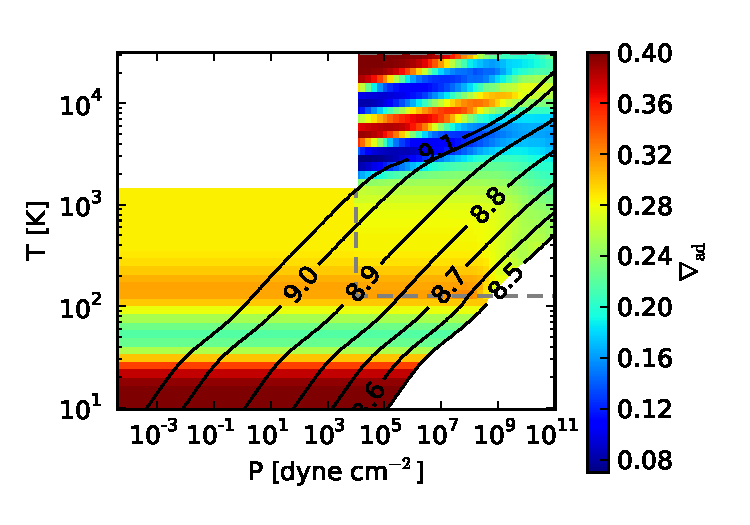
\includegraphics[scale=.8]{../../figs/ModelAtmospheres/RadSelfGravRealEOS/PaperFigs/delad_S_H.pdf}
\caption{Contour plot of the hydrogen adiabatic gradient $\delad$ as a function of gas temperature and pressure. The upper right rectangle encloses the region described by the original \citet{saumon95} EOS tables, while the rest of the plot is our extension to lower temperatures and pressures. The black curves represent constant entropy adiabats, with the labels the natural logarithm of the absolute entropy per unit mass. At high temperatures, hydrogen dissociates and ionizes, while at low temperatures the rotational states of the hydrogen molecule are only partially excited and it no longer behaves like an ideal diatomic gas. Regions in which the EOS is invalid or has not been computed are masked in white (see Figure \ref{fig:deladmap} caption for an explanation).}
\label{fig:deladH}
\end{figure}

\subsection{Helium}

We extend the helium EOS tables based on a similar procedure. Since helium is primarily neutral and atomic at low temperatures and pressures, we treat it as an ideal monoatomic gas, and thus only take into account the translational component of the partition function (\ref{eq:Zt}). Figure \ref{fig:deladHe} shows $\delad$ as a function of temperature and pressure for the extended EOS table. %The original and extended table join smoothly for entropy curves between $8.29<\log{S}$(K g$^{-1})<8.77$ in this case (\textbf{numbers are wrong, change once you have the final figure version}).

\begin{figure}[h!]
\centering
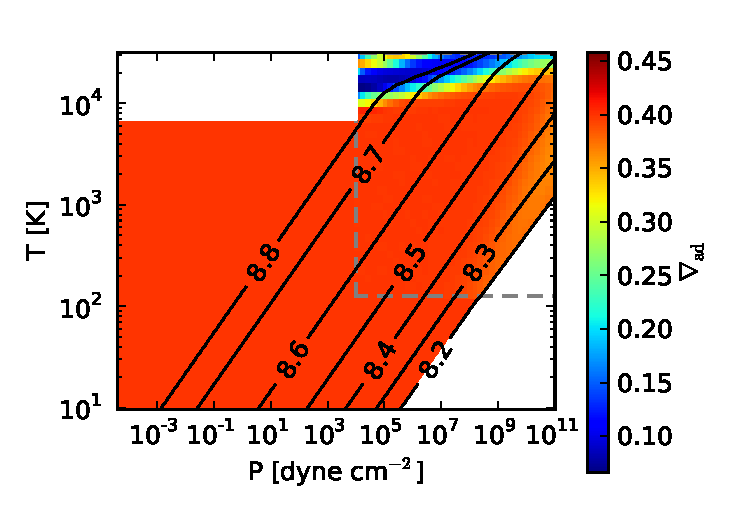
\includegraphics[scale=.8]{../../figs/ModelAtmospheres/RadSelfGravRealEOS/PaperFigs/delad_S_He.pdf}
\caption{Contour plot of the helium adiabatic gradient $\delad$ as a function of gas temperature and pressure. The upper right rectangle encloses the region described by the original \citet{saumon95} EOS tables, while the rest of the plot is our extension to lower temperatures and pressures. The black curves represent constant entropy adiabats, with the labels the natural logarithm of the absolute entropy per unit mass. Helium ionizes at $T \gtrsim 10,000$ K, but behaves as an ideal monatomic gas otherwise. We choose $T=7,000$ K as a conservative temperature cutoff above which our extension is no longer valid (masked in white). The EOS has not been computed in the lower-right region of the plot --- see Figure \ref{fig:deladmap} for an explanation.}
\label{fig:deladHe}
\end{figure}

\vspace{0.2in}

Lastly, we obtain the equation of state tables for the hydrogen-helium mixture thorough the procedure described in \citet{saumon95}, for a helium mass fraction $Y=0.3$.

%Using equation (\ref{eq:upartition}) we therefore recover the standard result $U_{\rm r}=\mathcal{R} T$ (refs). Furthermore, we know that the internal energy and entropy per unit mass associated with translation are given by $U_{\rm t}=\frac{3}{2} \mathcal{R}$ and $C_{\rm{v,t}}=\frac{3}{2}\mathcal{R}$, respectively, and so we are able to calculate the total internal energy and specific heat of a diatomic molecule as a function of temperature. An example of the variation of heat capacity with temperature is shown in \citet{kittel}, chapter 3. 

%The partition function associated with rotation is generally written as:
%
%\begin{equation}
%\label{eq:Zr}
%Z_{\rm r}=\sum_0^\infty (2 j +1) \exp\Big[-\frac{j(j+1)\Theta_r}{T}\Big],
%\end{equation}
%with $j$ the angular momentum quantum number \citep{kittel}. Various thermodynamic quantities can be derived from the partition function. For example, the internal energy per unit mass can be written as:
%
%\begin{equation}
%\label{eq:upartition}
%u_{\rm r}=\mathcal{R}T^2 \frac{\partial \log Z}{\partial T}
%\end{equation}
%
%The specific heat at constant volume then easily follows as
%
%\begin{equation}
%\label{eq:cvpartition}
%c_{\rm{v,r}}=\Big(\frac{\partial u}{\partial T}\Big)_V
%\end{equation} 


 







\section{Adiabatic Gradient during Partial Dissociation}\label{deladdiss}

%The adiabatic gradient during dissociation or ionization is a function of temperature and the dissociation or ionization fraction $x$. The Saha equation (e.g., \citealt{kippenhahn90}) relates $x$ to the gas 


The total internal energy of a partially dissociated gas includes contributions from the individual internal energies of the molecules and atoms, as well as from the dissociation energy. The dissociation energy depends on the dissociation fraction $x$ (i.e., the fraction of molecules that have dissociated), which can be found from the Saha equation (see e.g., \citealt{kippenhahn90}, Chapter 14) as a function of temperature and density,

\begin{equation}
\label{eq:saha}
\frac{x^2}{1-x} \propto \frac{T^{3/2}}{\rho} e^{-\chi/k_B T},
\end{equation} 
with $\chi$ the dissociation energy, equal to 4.48 eV for molecular hydrogen \citep{blanksby03}.

The above also holds true for ionization, with the dissociation energy replaced by ionization energy $\chi=13.6$ eV for atomic hydrogen \citep{mandl89}. From the Saha equation one can find an expression for $\rho$ as a function of $T$ and $x$, then derive the adiabatic gradient directly from its definition (equation \ref{eq:delad}), taking into account the fact that the mean molecular weight in the ideal gas law varies with $x$, hence the pressure will not only be a function of $T$ and $\rho$ but also of $x$ (see \citealt{kippenhahn90}, Chapter 14.3 for a detailed derivation). The final expression for the adiabatic gradient during ionization is 

\begin{equation}
\label{eq:deladioniz}
\delad=\frac{2+x (1-x) \Phi_H}{5+x(1-x)\Phi_H^2},
\end{equation}
with $\Phi_H \equiv \frac{5}{2}+\frac{\chi}{k_B T}$. The derivation of $\delad$ during dissociation is more involved mathematically (see, e.g., \citealt{vardya60}) and leads to a slightly more complicated final expression,

%One can derive a simple expression for the adiabatic gradient as a function of $x$ and $T$ from it's definition (equation \ref{eq:delad}), using the 

%The adiabatic gradient follows as (see \citealt{vardya60} for a detailed derivation)

\begin{equation}
\label{eq:deladdiss}
\delad=\frac{1+x+ \frac{x(1-x^2)}{2} \frac{\chi}{k_B T}}{5 x + \frac{7(1-x)}{2} + \frac{x(1-x^2)}{2} \Big(\frac{\chi}{k_B T}\Big)^2}.
\end{equation} 
We recover $\delad=2/7$ for $x=0$ (no ongoing dissociation hence hydrogen is purely molecular and diatomic) and $\delad=2/5$ for $x=1$ (hydrogen is fully dissociated into atoms and hence monatomic). Figure \ref{fig:deladdiss} shows the dependence of $\delad$ on the dissociation fraction, for $T=3000$ K, the temperature at which dissociation typically occurs \citep{langmuir12}. The adiabatic gradient drops substantially during partial dissociation, since part of the internal energy is used in dissociation rather than in increasing the temperature of the system.


\begin{figure}[h]
\centering
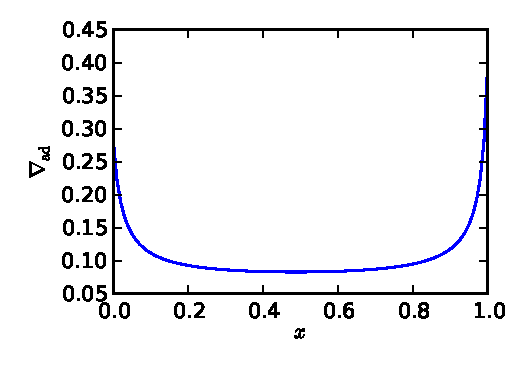
\includegraphics[width=0.5\textwidth]{../../figs/ModelAtmospheres/RadSelfGravRealEOS/PaperFigs/delad_dissociation.pdf}
%%\vspace{-0.5in}
\caption{Adiabatic gradient as a function of the hydrogen dissociation fraction $x$. The adiabatic gradient is $\delad=2/7$ for pure molecular hydrogen ($x=0$) and $\delad=2/5$ for fully atomic hydrogen ($x=1$), and drops to low values during partial dissociation.}
\label{fig:deladdiss}
\end{figure}


%with $\chi$ and $T$ the dissociation energy and temperature, respectively, equal to $\chi=4.48$ eV\citep{blanksby03} and $T\sim3000$ K \citep{langmuir12} for molecular hydrogen.

%Specifically, if we denote the internal energies of neutral hydrogen, protons and electrons as $U_{H}$, $U_+$ and $U_e$, respectively, then the total internal energy of the gas is given by:

%\begin{equation}
%U=U_H+U_+ + U_e + x \chi,
%\end{equation}
%
%\noindent where $x$ is the ionization fraction and $\chi$ is the ionization energy (equal to -13.6 eV for hydrogen). The ionization fraction can be determined from the Saha equation (see e.g., \citealt{kippenhahn90}).
%
%\begin{equation}
%\label{eq:saha}
%\frac{x^2}{1-x} \frac{\rho}{m_H}=\frac{(2 \pi m_e k_B T)^{3/2}}{h^3} e^{-\chi/k_B T},
%\end{equation}
%
%\noindent where $m_e$ is the mass of the electron and $h$ is Planck's constant. It can be seen from the Saha equation that the ionization fraction depends only on the gas temperature and density: $x=x(T, \rho)$. As such, all the thermodynamic quantities also depend only on the gas temperature and density, and hence on the equation of state. The adiabatic gradient is given by (see \citealt{kippenhahn90}, chapter 14 for a derivation):
%
%\begin{equation}
%\delad=\frac{2+x (1-x) \Phi_H}{5+x (1-x) \Phi_H^2},
%\end{equation} 
%with $\Phi_H=\frac{5}{2}+\frac{\chi}{k T}$. Figure \ref{fig:deladion} shows the behavior of $\delad$ for partially ionized hydrogen. We recover $\delad=2/5$ for $x=0$ (pure atomic hydrogen) and $x=1$ (fully ionized plasma). The adiabatic gradient decreases significantly for intermediate values of $x$, becoming smaller than 0.1 at its minimum (for $x=0.5$). 

\section{Grain growth opacity and radiative windows} \label{radwindow}

The opacity of the interstellar medium is reasonably well constrained and approximate analytic expressions for the Rosseland mean opacity as a function of temperature and density are derived in \citet{bell94}. For low temperatures ($T \lesssim 100$ K) at which ice grains are present, opacity scales with temperature as $\kappa \sim T^2$. Sublimation of ice grains at $\sim 150$ K and of metal grains at $\sim 1000$ K results in sharp opacity drops. This is shown in Figure \ref{fig:opacity} for a gas density $\rho=10^{-8}$ g cm$^{-3}$, which is typical for the outer regions of protoplanetary disks. \citet{semenov03} calculate Rosseland mean opacities in protoplanetary disks for grains of different sizes and structure. As shown in Figure \ref{fig:opacity}, their results are in good agreement with \citet{bell94}. However, \citet{semenov03} do not take grain growth into account, which is likely to occur in protoplanetary disks, particularly when most solids have been accreted. \citet{dalessio01} compute wavelength dependent opacities for a range of maximum particle sizes and different size distributions. Figure \ref{fig:opacity} shows the integrated Rosseland mean opacity for a maximum particle size of 1 cm and a power law size distribution $n \sim a^{-p}$, with $a$ the grain size and $p=3.5$ for a normal collisional cascade and $p=2.5$ when coagulation is taken into account. We see in Figure \ref{fig:opacity} that this yields a mean opacity that is both lower and less sensitive to temperature, when compared to \citet{bell94} or \citet{semenov03}. However, observations of dust in protoplanetary disks have only been made at low temperatures (i.e., before dust sublimates). As we see in Figure \ref{fig:opacity}, the opacity dramatically decreases during dust sublimation for ISM grains, which can result in regions in the inner parts of planetary atmospheres where energy is transported radiatively, i.e. radiative windows. We thus use the \citet{bell94} opacities for $T \gtrsim 1000$ K, ensuring they smoothly match the \citet{dalessio01} opacities for lower temperatures.

\begin{figure}[h!]
\centering
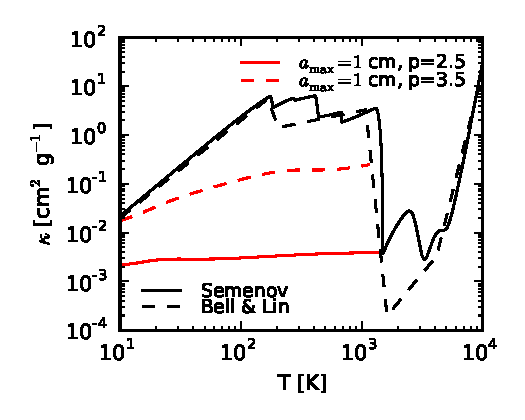
\includegraphics[width=0.5\textwidth]{../../figs/ModelAtmospheres/RadSelfGravRealEOS/PaperFigs/kappa_grain_growth_SBL_paper.pdf}
%%\vspace{-0.5in}
\caption{Rosseland mean opacity of dust grains as a function of temperature for different opacity assumptions. The dashed black curve shows the \citet{bell94} analytic ISM opacity for $\rho=10^{-8}$ g cm$^{-3}$. The solid black curve shows the tabulated opacity of \citet{semenov03} for a dust composition of 'normal' silicates. The dashed red curve shows the \citet{dalessio01} opacity, which takes grain growth into account, for a maximum particle size of 1 cm and a normal collisional cascade grain size distribution ($p=3.5$). The solid red curve is the same as the dashed red curve, but it accounts for coagulation ($p=2.5$).}
\label{fig:opacity}
\end{figure}

The significant opacity drop due to the sublimation of ice and metal grains lowers the radiative temperature gradient $\delrad$, which may result in one or more inner radiative layers inside the atmosphere of a protoplanet. This is displayed in Figure \ref{fig:delvsr}: depending on the semi-major axis and core mass, the opacity drop will generate no radiative window (top panel), one radiative window (middle panel), or two radiative windows (bottom panel). 

\begin{figure}[h!]
\centering
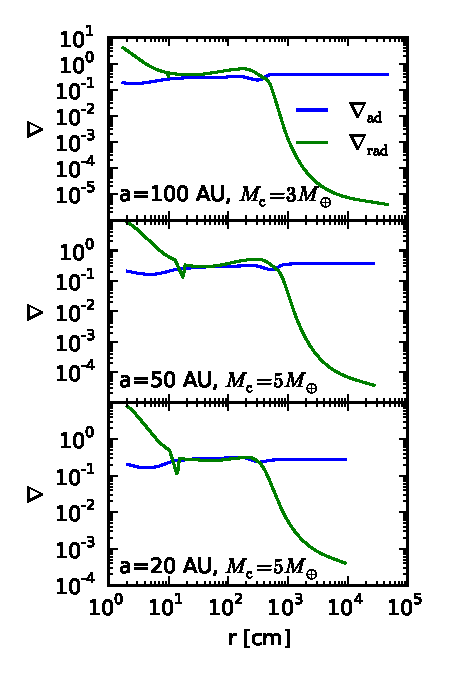
\includegraphics[width=0.5\textwidth]{../../figs/ModelAtmospheres/RadSelfGravRealEOS/Opacity/del_vs_r.pdf}
%%\vspace{-0.5in}
\caption{Snapshots of the radiative and adiabatic gradient as a function of the radial coordinate, for planets with different core masses forming at various locations in the disk. The sharp drop in opacity due to dust sublimation may generate one or more radiative windows. Top panel: no radiative window for $a=100$ AU and $M\co=3 M_{\oplus}$. Middle panel: the opacity drop produces one radiative window for $a=50$ AU and $M\co=5 M_{\oplus}$. Bottom panel: the sharp drop in opacity results in two radiative windows for $a=20$ AU and $M\co=3 M_{\oplus}$.}
\label{fig:delvsr}
\end{figure}



\end{document}




